\documentclass[10pt,]{article}
\usepackage{lmodern}
\usepackage{amssymb,amsmath}
\usepackage{ifxetex,ifluatex}
\usepackage{fixltx2e} % provides \textsubscript
\ifnum 0\ifxetex 1\fi\ifluatex 1\fi=0 % if pdftex
  \usepackage[T1]{fontenc}
  \usepackage[utf8]{inputenc}
\else % if luatex or xelatex
  \ifxetex
    \usepackage{mathspec}
  \else
    \usepackage{fontspec}
  \fi
  \defaultfontfeatures{Ligatures=TeX,Scale=MatchLowercase}
\fi
% use upquote if available, for straight quotes in verbatim environments
\IfFileExists{upquote.sty}{\usepackage{upquote}}{}
% use microtype if available
\IfFileExists{microtype.sty}{%
\usepackage{microtype}
\UseMicrotypeSet[protrusion]{basicmath} % disable protrusion for tt fonts
}{}
\usepackage[margin=2cm]{geometry}
\usepackage{hyperref}
\hypersetup{unicode=true,
            pdftitle={Lathyrus - Weather},
            pdfborder={0 0 0},
            breaklinks=true}
\urlstyle{same}  % don't use monospace font for urls
\usepackage{color}
\usepackage{fancyvrb}
\newcommand{\VerbBar}{|}
\newcommand{\VERB}{\Verb[commandchars=\\\{\}]}
\DefineVerbatimEnvironment{Highlighting}{Verbatim}{commandchars=\\\{\}}
% Add ',fontsize=\small' for more characters per line
\usepackage{framed}
\definecolor{shadecolor}{RGB}{248,248,248}
\newenvironment{Shaded}{\begin{snugshade}}{\end{snugshade}}
\newcommand{\KeywordTok}[1]{\textcolor[rgb]{0.13,0.29,0.53}{\textbf{#1}}}
\newcommand{\DataTypeTok}[1]{\textcolor[rgb]{0.13,0.29,0.53}{#1}}
\newcommand{\DecValTok}[1]{\textcolor[rgb]{0.00,0.00,0.81}{#1}}
\newcommand{\BaseNTok}[1]{\textcolor[rgb]{0.00,0.00,0.81}{#1}}
\newcommand{\FloatTok}[1]{\textcolor[rgb]{0.00,0.00,0.81}{#1}}
\newcommand{\ConstantTok}[1]{\textcolor[rgb]{0.00,0.00,0.00}{#1}}
\newcommand{\CharTok}[1]{\textcolor[rgb]{0.31,0.60,0.02}{#1}}
\newcommand{\SpecialCharTok}[1]{\textcolor[rgb]{0.00,0.00,0.00}{#1}}
\newcommand{\StringTok}[1]{\textcolor[rgb]{0.31,0.60,0.02}{#1}}
\newcommand{\VerbatimStringTok}[1]{\textcolor[rgb]{0.31,0.60,0.02}{#1}}
\newcommand{\SpecialStringTok}[1]{\textcolor[rgb]{0.31,0.60,0.02}{#1}}
\newcommand{\ImportTok}[1]{#1}
\newcommand{\CommentTok}[1]{\textcolor[rgb]{0.56,0.35,0.01}{\textit{#1}}}
\newcommand{\DocumentationTok}[1]{\textcolor[rgb]{0.56,0.35,0.01}{\textbf{\textit{#1}}}}
\newcommand{\AnnotationTok}[1]{\textcolor[rgb]{0.56,0.35,0.01}{\textbf{\textit{#1}}}}
\newcommand{\CommentVarTok}[1]{\textcolor[rgb]{0.56,0.35,0.01}{\textbf{\textit{#1}}}}
\newcommand{\OtherTok}[1]{\textcolor[rgb]{0.56,0.35,0.01}{#1}}
\newcommand{\FunctionTok}[1]{\textcolor[rgb]{0.00,0.00,0.00}{#1}}
\newcommand{\VariableTok}[1]{\textcolor[rgb]{0.00,0.00,0.00}{#1}}
\newcommand{\ControlFlowTok}[1]{\textcolor[rgb]{0.13,0.29,0.53}{\textbf{#1}}}
\newcommand{\OperatorTok}[1]{\textcolor[rgb]{0.81,0.36,0.00}{\textbf{#1}}}
\newcommand{\BuiltInTok}[1]{#1}
\newcommand{\ExtensionTok}[1]{#1}
\newcommand{\PreprocessorTok}[1]{\textcolor[rgb]{0.56,0.35,0.01}{\textit{#1}}}
\newcommand{\AttributeTok}[1]{\textcolor[rgb]{0.77,0.63,0.00}{#1}}
\newcommand{\RegionMarkerTok}[1]{#1}
\newcommand{\InformationTok}[1]{\textcolor[rgb]{0.56,0.35,0.01}{\textbf{\textit{#1}}}}
\newcommand{\WarningTok}[1]{\textcolor[rgb]{0.56,0.35,0.01}{\textbf{\textit{#1}}}}
\newcommand{\AlertTok}[1]{\textcolor[rgb]{0.94,0.16,0.16}{#1}}
\newcommand{\ErrorTok}[1]{\textcolor[rgb]{0.64,0.00,0.00}{\textbf{#1}}}
\newcommand{\NormalTok}[1]{#1}
\usepackage{longtable,booktabs}
\usepackage{graphicx,grffile}
\makeatletter
\def\maxwidth{\ifdim\Gin@nat@width>\linewidth\linewidth\else\Gin@nat@width\fi}
\def\maxheight{\ifdim\Gin@nat@height>\textheight\textheight\else\Gin@nat@height\fi}
\makeatother
% Scale images if necessary, so that they will not overflow the page
% margins by default, and it is still possible to overwrite the defaults
% using explicit options in \includegraphics[width, height, ...]{}
\setkeys{Gin}{width=\maxwidth,height=\maxheight,keepaspectratio}
\IfFileExists{parskip.sty}{%
\usepackage{parskip}
}{% else
\setlength{\parindent}{0pt}
\setlength{\parskip}{6pt plus 2pt minus 1pt}
}
\setlength{\emergencystretch}{3em}  % prevent overfull lines
\providecommand{\tightlist}{%
  \setlength{\itemsep}{0pt}\setlength{\parskip}{0pt}}
\setcounter{secnumdepth}{0}
% Redefines (sub)paragraphs to behave more like sections
\ifx\paragraph\undefined\else
\let\oldparagraph\paragraph
\renewcommand{\paragraph}[1]{\oldparagraph{#1}\mbox{}}
\fi
\ifx\subparagraph\undefined\else
\let\oldsubparagraph\subparagraph
\renewcommand{\subparagraph}[1]{\oldsubparagraph{#1}\mbox{}}
\fi

%%% Use protect on footnotes to avoid problems with footnotes in titles
\let\rmarkdownfootnote\footnote%
\def\footnote{\protect\rmarkdownfootnote}

%%% Change title format to be more compact
\usepackage{titling}

% Create subtitle command for use in maketitle
\newcommand{\subtitle}[1]{
  \posttitle{
    \begin{center}\large#1\end{center}
    }
}

\setlength{\droptitle}{-2em}
  \title{Lathyrus - Weather}
  \pretitle{\vspace{\droptitle}\centering\huge}
  \posttitle{\par}
  \author{}
  \preauthor{}\postauthor{}
  \date{}
  \predate{}\postdate{}


\begin{document}
\maketitle

Temperature and precipitation data\\
Temperature (daily mean, minimum and maximum) from two stations:
Oxelösund and Södertalje\\
Precipitation from one station: Åda

\begin{longtable}[]{@{}llrrrrlrlrl@{}}
\toprule
station & date & year & month & day & mean & quality\_mean & min &
quality\_.min & max & quality\_max\tabularnewline
\midrule
\endhead
Oxelösund & 1987-01-01 & 1987 & 1 & 1 & -11.6 & Y & -14.5 & G & -9.0 &
G\tabularnewline
Oxelösund & 1987-01-02 & 1987 & 1 & 2 & -10.4 & Y & -16.5 & G & -7.8 &
G\tabularnewline
Oxelösund & 1987-01-03 & 1987 & 1 & 3 & -9.9 & Y & -11.8 & G & -8.3 &
G\tabularnewline
Oxelösund & 1987-01-04 & 1987 & 1 & 4 & -14.1 & Y & -17.0 & G & -10.4 &
G\tabularnewline
Oxelösund & 1987-01-05 & 1987 & 1 & 5 & -4.6 & Y & -17.0 & G & -1.5 &
G\tabularnewline
Oxelösund & 1987-01-06 & 1987 & 1 & 6 & -10.7 & Y & -14.5 & G & -3.0 &
G\tabularnewline
\bottomrule
\end{longtable}

\begin{longtable}[]{@{}llrrrrl@{}}
\toprule
station & date & year & month & day & precipitation &
quality\tabularnewline
\midrule
\endhead
Åda & 1987-01-01 & 1987 & 1 & 1 & 0.0 & Y\tabularnewline
Åda & 1987-01-02 & 1987 & 1 & 2 & 0.0 & Y\tabularnewline
Åda & 1987-01-03 & 1987 & 1 & 3 & 0.3 & Y\tabularnewline
Åda & 1987-01-04 & 1987 & 1 & 4 & 1.1 & Y\tabularnewline
Åda & 1987-01-05 & 1987 & 1 & 5 & 0.0 & Y\tabularnewline
Åda & 1987-01-06 & 1987 & 1 & 6 & 2.8 & Y\tabularnewline
\bottomrule
\end{longtable}

Distributions

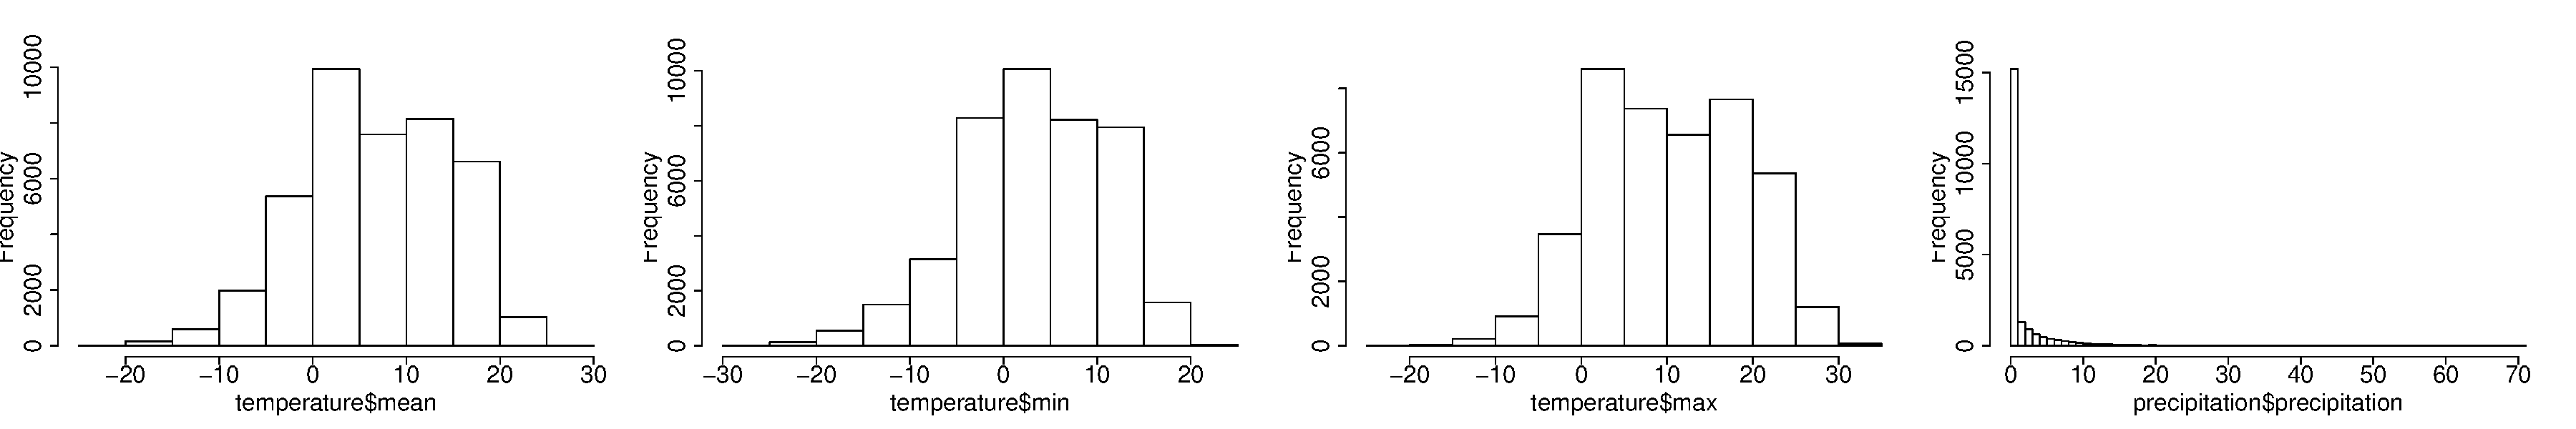
\includegraphics{weather_nb_files/figure-latex/Distributions-1.pdf}

Boxplots per month

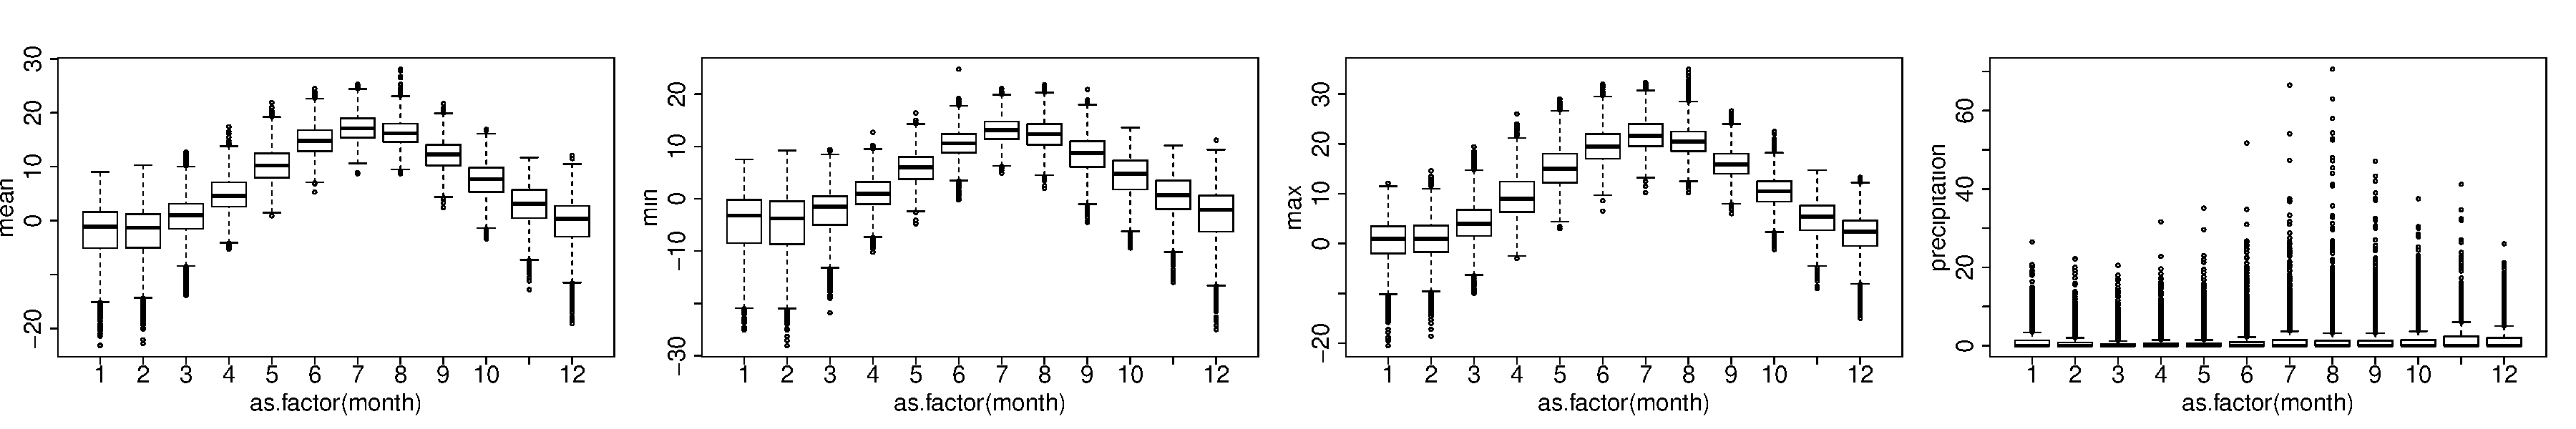
\includegraphics{weather_nb_files/figure-latex/Boxplots per month-1.pdf}

\newpage

Comparisons of mean temperatures for each year for both stations: they
look quite similar

\includegraphics{weather_nb_files/figure-latex/Graph mean temperatures for each year for both stations-1.pdf}

Temperature: average mean, min and max of the two stations for further
use + join with precipitation data

\begin{longtable}[]{@{}lrrrlrrrr@{}}
\toprule
date & year & month & day & date\_ok & mean & min & max &
precipitation\tabularnewline
\midrule
\endhead
1987-01-01 & 1987 & 1 & 1 & 01/01/1987 & -11.25 & -14.15 & -8.50 &
0.0\tabularnewline
1987-01-02 & 1987 & 1 & 2 & 02/01/1987 & -11.50 & -15.25 & -7.65 &
0.0\tabularnewline
1987-01-03 & 1987 & 1 & 3 & 03/01/1987 & -10.25 & -14.40 & -7.90 &
0.3\tabularnewline
1987-01-04 & 1987 & 1 & 4 & 04/01/1987 & -13.35 & -16.25 & -9.20 &
1.1\tabularnewline
1987-01-05 & 1987 & 1 & 5 & 05/01/1987 & -5.95 & -16.50 & -2.50 &
0.0\tabularnewline
1987-01-06 & 1987 & 1 & 6 & 06/01/1987 & -11.85 & -15.25 & -4.25 &
2.8\tabularnewline
\bottomrule
\end{longtable}

\begin{Shaded}
\begin{Highlighting}[]
\KeywordTok{nrow}\NormalTok{(}\KeywordTok{subset}\NormalTok{(weather,}\KeywordTok{is.na}\NormalTok{(precipitation))) }\CommentTok{#154 dates with missing precipitation}
\end{Highlighting}
\end{Shaded}

\begin{verbatim}
## [1] 154
\end{verbatim}

\begin{Shaded}
\begin{Highlighting}[]
\KeywordTok{unique}\NormalTok{(}\KeywordTok{subset}\NormalTok{(weather,}\KeywordTok{is.na}\NormalTok{(precipitation))[}\DecValTok{2}\OperatorTok{:}\DecValTok{3}\NormalTok{]) }\CommentTok{#See which years/months}
\end{Highlighting}
\end{Shaded}

\begin{verbatim}
##      year month
## 397  1988     2
## 1613 1991     6
## 1858 1992     2
## 2101 1992    10
## 7970 2017    10
## 7976 2017    11
\end{verbatim}

\begin{Shaded}
\begin{Highlighting}[]
\CommentTok{#February 1988, June 1991, February 1992, October 1992 all missing}
\CommentTok{#Substitute with mean of all years for each specific date}
\NormalTok{weather}\OperatorTok{$}\NormalTok{precipitation[}\KeywordTok{is.na}\NormalTok{(weather}\OperatorTok{$}\NormalTok{precipitation)}\OperatorTok{&}\NormalTok{weather}\OperatorTok{$}\NormalTok{year}\OperatorTok{==}\DecValTok{1988}\OperatorTok{&}\NormalTok{weather}\OperatorTok{$}\NormalTok{month}\OperatorTok{==}\DecValTok{2}\NormalTok{]<-}
\StringTok{  }\KeywordTok{with}\NormalTok{(}\KeywordTok{subset}\NormalTok{(}\KeywordTok{aggregate}\NormalTok{(precipitation }\OperatorTok{~}\StringTok{ }\NormalTok{year}\OperatorTok{+}\NormalTok{month}\OperatorTok{+}\NormalTok{day, }\DataTypeTok{data=}\NormalTok{ weather, }\DataTypeTok{FUN=}\NormalTok{sum),month}\OperatorTok{==}\DecValTok{2}\NormalTok{),}
  \KeywordTok{aggregate}\NormalTok{(precipitation}\OperatorTok{~}\NormalTok{day,}\DataTypeTok{FUN=}\NormalTok{mean)}\OperatorTok{$}\NormalTok{precipitation) }
\NormalTok{weather}\OperatorTok{$}\NormalTok{precipitation[}\KeywordTok{is.na}\NormalTok{(weather}\OperatorTok{$}\NormalTok{precipitation)}\OperatorTok{&}\NormalTok{weather}\OperatorTok{$}\NormalTok{year}\OperatorTok{==}\DecValTok{1991}\OperatorTok{&}\NormalTok{weather}\OperatorTok{$}\NormalTok{month}\OperatorTok{==}\DecValTok{6}\NormalTok{]<-}
\StringTok{  }\KeywordTok{with}\NormalTok{(}\KeywordTok{subset}\NormalTok{(}\KeywordTok{aggregate}\NormalTok{(precipitation }\OperatorTok{~}\StringTok{ }\NormalTok{year}\OperatorTok{+}\NormalTok{month}\OperatorTok{+}\NormalTok{day, }\DataTypeTok{data=}\NormalTok{ weather, }\DataTypeTok{FUN=}\NormalTok{sum),month}\OperatorTok{==}\DecValTok{6}\NormalTok{),}
  \KeywordTok{aggregate}\NormalTok{(precipitation}\OperatorTok{~}\NormalTok{day,}\DataTypeTok{FUN=}\NormalTok{mean)}\OperatorTok{$}\NormalTok{precipitation) }
\NormalTok{weather}\OperatorTok{$}\NormalTok{precipitation[}\KeywordTok{is.na}\NormalTok{(weather}\OperatorTok{$}\NormalTok{precipitation)}\OperatorTok{&}\NormalTok{weather}\OperatorTok{$}\NormalTok{year}\OperatorTok{==}\DecValTok{1992}\OperatorTok{&}\NormalTok{weather}\OperatorTok{$}\NormalTok{month}\OperatorTok{==}\DecValTok{2}\NormalTok{]<-}
\StringTok{  }\KeywordTok{with}\NormalTok{(}\KeywordTok{subset}\NormalTok{(}\KeywordTok{aggregate}\NormalTok{(precipitation }\OperatorTok{~}\StringTok{ }\NormalTok{year}\OperatorTok{+}\NormalTok{month}\OperatorTok{+}\NormalTok{day, }\DataTypeTok{data=}\NormalTok{ weather, }\DataTypeTok{FUN=}\NormalTok{sum),month}\OperatorTok{==}\DecValTok{2}\NormalTok{),}
  \KeywordTok{aggregate}\NormalTok{(precipitation}\OperatorTok{~}\NormalTok{day,}\DataTypeTok{FUN=}\NormalTok{mean)}\OperatorTok{$}\NormalTok{precipitation) }
\NormalTok{weather}\OperatorTok{$}\NormalTok{precipitation[}\KeywordTok{is.na}\NormalTok{(weather}\OperatorTok{$}\NormalTok{precipitation)}\OperatorTok{&}\NormalTok{weather}\OperatorTok{$}\NormalTok{year}\OperatorTok{==}\DecValTok{1992}\OperatorTok{&}\NormalTok{weather}\OperatorTok{$}\NormalTok{month}\OperatorTok{==}\DecValTok{10}\NormalTok{]<-}
\StringTok{  }\KeywordTok{with}\NormalTok{(}\KeywordTok{subset}\NormalTok{(}\KeywordTok{aggregate}\NormalTok{(precipitation }\OperatorTok{~}\StringTok{ }\NormalTok{year}\OperatorTok{+}\NormalTok{month}\OperatorTok{+}\NormalTok{day, }\DataTypeTok{data=}\NormalTok{ weather, }\DataTypeTok{FUN=}\NormalTok{sum),month}\OperatorTok{==}\DecValTok{10}\NormalTok{),}
  \KeywordTok{aggregate}\NormalTok{(precipitation}\OperatorTok{~}\NormalTok{day,}\DataTypeTok{FUN=}\NormalTok{mean)}\OperatorTok{$}\NormalTok{precipitation) }
\CommentTok{#October-November 2017 leave as NAs, will be available later}
\end{Highlighting}
\end{Shaded}

Calculation of GDD and GDH (base =3/5/7/10 ºC)\\
GDD:\\
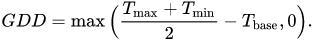
\includegraphics{C:/Users/User/Dropbox/SU/Projects/lathyrus/code/GDD.png}

GDH:\\
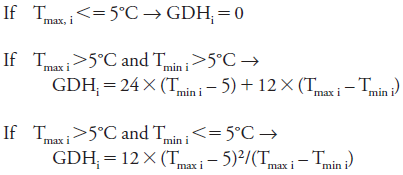
\includegraphics{C:/Users/User/Dropbox/SU/Projects/lathyrus/code/GDH.png}

\begin{Shaded}
\begin{Highlighting}[]
\NormalTok{weather}\OperatorTok{$}\NormalTok{GDD3<-}\KeywordTok{ifelse}\NormalTok{(}\KeywordTok{with}\NormalTok{(weather,((max}\OperatorTok{+}\NormalTok{min)}\OperatorTok{/}\DecValTok{2}\NormalTok{)}\OperatorTok{-}\DecValTok{3}\NormalTok{)}\OperatorTok{<}\DecValTok{0}\NormalTok{,}\DecValTok{0}\NormalTok{,}\KeywordTok{with}\NormalTok{(weather,((max}\OperatorTok{+}\NormalTok{min)}\OperatorTok{/}\DecValTok{2}\NormalTok{)}\OperatorTok{-}\DecValTok{3}\NormalTok{))}
\NormalTok{weather}\OperatorTok{$}\NormalTok{GDD5<-}\KeywordTok{ifelse}\NormalTok{(}\KeywordTok{with}\NormalTok{(weather,((max}\OperatorTok{+}\NormalTok{min)}\OperatorTok{/}\DecValTok{2}\NormalTok{)}\OperatorTok{-}\DecValTok{5}\NormalTok{)}\OperatorTok{<}\DecValTok{0}\NormalTok{,}\DecValTok{0}\NormalTok{,}\KeywordTok{with}\NormalTok{(weather,((max}\OperatorTok{+}\NormalTok{min)}\OperatorTok{/}\DecValTok{2}\NormalTok{)}\OperatorTok{-}\DecValTok{5}\NormalTok{))}
\NormalTok{weather}\OperatorTok{$}\NormalTok{GDD7<-}\KeywordTok{ifelse}\NormalTok{(}\KeywordTok{with}\NormalTok{(weather,((max}\OperatorTok{+}\NormalTok{min)}\OperatorTok{/}\DecValTok{2}\NormalTok{)}\OperatorTok{-}\DecValTok{7}\NormalTok{)}\OperatorTok{<}\DecValTok{0}\NormalTok{,}\DecValTok{0}\NormalTok{,}\KeywordTok{with}\NormalTok{(weather,((max}\OperatorTok{+}\NormalTok{min)}\OperatorTok{/}\DecValTok{2}\NormalTok{)}\OperatorTok{-}\DecValTok{7}\NormalTok{))}
\NormalTok{weather}\OperatorTok{$}\NormalTok{GDD10<-}\KeywordTok{ifelse}\NormalTok{(}\KeywordTok{with}\NormalTok{(weather,((max}\OperatorTok{+}\NormalTok{min)}\OperatorTok{/}\DecValTok{2}\NormalTok{)}\OperatorTok{-}\DecValTok{10}\NormalTok{)}\OperatorTok{<}\DecValTok{0}\NormalTok{,}\DecValTok{0}\NormalTok{,}\KeywordTok{with}\NormalTok{(weather,((max}\OperatorTok{+}\NormalTok{min)}\OperatorTok{/}\DecValTok{2}\NormalTok{)}\OperatorTok{-}\DecValTok{10}\NormalTok{))}

\NormalTok{weather}\OperatorTok{$}\NormalTok{GDH3<-}\KeywordTok{ifelse}\NormalTok{(}\KeywordTok{with}\NormalTok{(weather,max}\OperatorTok{<=}\DecValTok{3}\NormalTok{),}\DecValTok{0}\NormalTok{,}
                     \KeywordTok{ifelse}\NormalTok{(}\KeywordTok{with}\NormalTok{(weather,max}\OperatorTok{>}\DecValTok{3}\OperatorTok{&}\NormalTok{min}\OperatorTok{>}\DecValTok{3}\NormalTok{),}\KeywordTok{with}\NormalTok{(weather,}\DecValTok{24}\OperatorTok{*}\NormalTok{(min}\OperatorTok{-}\DecValTok{3}\NormalTok{)}\OperatorTok{+}\DecValTok{12}\OperatorTok{*}\NormalTok{(max}\OperatorTok{-}\NormalTok{min)),}
                            \KeywordTok{with}\NormalTok{(weather,}\DecValTok{12}\OperatorTok{*}\NormalTok{(max}\OperatorTok{-}\DecValTok{3}\NormalTok{)}\OperatorTok{^}\DecValTok{2}\OperatorTok{/}\NormalTok{(max}\OperatorTok{-}\NormalTok{min))))}
\NormalTok{weather}\OperatorTok{$}\NormalTok{GDH5<-}\KeywordTok{ifelse}\NormalTok{(}\KeywordTok{with}\NormalTok{(weather,max}\OperatorTok{<=}\DecValTok{5}\NormalTok{),}\DecValTok{0}\NormalTok{,}
                     \KeywordTok{ifelse}\NormalTok{(}\KeywordTok{with}\NormalTok{(weather,max}\OperatorTok{>}\DecValTok{5}\OperatorTok{&}\NormalTok{min}\OperatorTok{>}\DecValTok{5}\NormalTok{),}\KeywordTok{with}\NormalTok{(weather,}\DecValTok{24}\OperatorTok{*}\NormalTok{(min}\OperatorTok{-}\DecValTok{5}\NormalTok{)}\OperatorTok{+}\DecValTok{12}\OperatorTok{*}\NormalTok{(max}\OperatorTok{-}\NormalTok{min)),}
                            \KeywordTok{with}\NormalTok{(weather,}\DecValTok{12}\OperatorTok{*}\NormalTok{(max}\OperatorTok{-}\DecValTok{5}\NormalTok{)}\OperatorTok{^}\DecValTok{2}\OperatorTok{/}\NormalTok{(max}\OperatorTok{-}\NormalTok{min))))}
\NormalTok{weather}\OperatorTok{$}\NormalTok{GDH7<-}\KeywordTok{ifelse}\NormalTok{(}\KeywordTok{with}\NormalTok{(weather,max}\OperatorTok{<=}\DecValTok{7}\NormalTok{),}\DecValTok{0}\NormalTok{,}
                     \KeywordTok{ifelse}\NormalTok{(}\KeywordTok{with}\NormalTok{(weather,max}\OperatorTok{>}\DecValTok{7}\OperatorTok{&}\NormalTok{min}\OperatorTok{>}\DecValTok{7}\NormalTok{),}\KeywordTok{with}\NormalTok{(weather,}\DecValTok{24}\OperatorTok{*}\NormalTok{(min}\OperatorTok{-}\DecValTok{7}\NormalTok{)}\OperatorTok{+}\DecValTok{12}\OperatorTok{*}\NormalTok{(max}\OperatorTok{-}\NormalTok{min)),}
                            \KeywordTok{with}\NormalTok{(weather,}\DecValTok{12}\OperatorTok{*}\NormalTok{(max}\OperatorTok{-}\DecValTok{7}\NormalTok{)}\OperatorTok{^}\DecValTok{2}\OperatorTok{/}\NormalTok{(max}\OperatorTok{-}\NormalTok{min))))}
\NormalTok{weather}\OperatorTok{$}\NormalTok{GDH10<-}\KeywordTok{ifelse}\NormalTok{(}\KeywordTok{with}\NormalTok{(weather,max}\OperatorTok{<=}\DecValTok{10}\NormalTok{),}\DecValTok{0}\NormalTok{,}
                     \KeywordTok{ifelse}\NormalTok{(}\KeywordTok{with}\NormalTok{(weather,max}\OperatorTok{>}\DecValTok{10}\OperatorTok{&}\NormalTok{min}\OperatorTok{>}\DecValTok{10}\NormalTok{),}\KeywordTok{with}\NormalTok{(weather,}\DecValTok{24}\OperatorTok{*}\NormalTok{(min}\OperatorTok{-}\DecValTok{10}\NormalTok{)}\OperatorTok{+}\DecValTok{12}\OperatorTok{*}\NormalTok{(max}\OperatorTok{-}\NormalTok{min)),}
                            \KeywordTok{with}\NormalTok{(weather,}\DecValTok{12}\OperatorTok{*}\NormalTok{(max}\OperatorTok{-}\DecValTok{10}\NormalTok{)}\OperatorTok{^}\DecValTok{2}\OperatorTok{/}\NormalTok{(max}\OperatorTok{-}\NormalTok{min))))}
\KeywordTok{pander}\NormalTok{(}\KeywordTok{head}\NormalTok{(weather), }\DataTypeTok{split.table =} \DecValTok{100}\NormalTok{, }\DataTypeTok{style =} \StringTok{'rmarkdown'}\NormalTok{)}
\end{Highlighting}
\end{Shaded}

\begin{longtable}[]{@{}ccccccccc@{}}
\toprule
date & year & month & day & date\_ok & mean & min & max &
precipitation\tabularnewline
\midrule
\endhead
1987-01-01 & 1987 & 1 & 1 & 01/01/1987 & -11.25 & -14.15 & -8.5 &
0\tabularnewline
1987-01-02 & 1987 & 1 & 2 & 02/01/1987 & -11.5 & -15.25 & -7.65 &
0\tabularnewline
1987-01-03 & 1987 & 1 & 3 & 03/01/1987 & -10.25 & -14.4 & -7.9 &
0.3\tabularnewline
1987-01-04 & 1987 & 1 & 4 & 04/01/1987 & -13.35 & -16.25 & -9.2 &
1.1\tabularnewline
1987-01-05 & 1987 & 1 & 5 & 05/01/1987 & -5.95 & -16.5 & -2.5 &
0\tabularnewline
1987-01-06 & 1987 & 1 & 6 & 06/01/1987 & -11.85 & -15.25 & -4.25 &
2.8\tabularnewline
\bottomrule
\end{longtable}

\begin{longtable}[]{@{}cccccccc@{}}
\toprule
GDD3 & GDD5 & GDD7 & GDD10 & GDH3 & GDH5 & GDH7 & GDH10\tabularnewline
\midrule
\endhead
0 & 0 & 0 & 0 & 0 & 0 & 0 & 0\tabularnewline
0 & 0 & 0 & 0 & 0 & 0 & 0 & 0\tabularnewline
0 & 0 & 0 & 0 & 0 & 0 & 0 & 0\tabularnewline
0 & 0 & 0 & 0 & 0 & 0 & 0 & 0\tabularnewline
0 & 0 & 0 & 0 & 0 & 0 & 0 & 0\tabularnewline
0 & 0 & 0 & 0 & 0 & 0 & 0 & 0\tabularnewline
\bottomrule
\end{longtable}

Define 3 periods:\\
a) Before vernal equinox (March 20-21 depending on the year)\\
b) From vernal equinox to 60 days after\\
c) 61+ days after vernal equinox (May 20-21 depending on the year)

\begin{Shaded}
\begin{Highlighting}[]
\NormalTok{weather<-}\KeywordTok{merge}\NormalTok{(weather,}\KeywordTok{unique}\NormalTok{(alldata[}\KeywordTok{c}\NormalTok{(}\DecValTok{1}\NormalTok{,}\DecValTok{8}\NormalTok{)])) }\CommentTok{#Add column with date of vernal equinox}
\NormalTok{weather}\OperatorTok{$}\NormalTok{vernal_time<-}\KeywordTok{as.POSIXct}\NormalTok{(weather}\OperatorTok{$}\NormalTok{vernal,}\DataTypeTok{format=}\StringTok{"%d/%m/%y %H:%M"}\NormalTok{)}
\NormalTok{weather}\OperatorTok{$}\NormalTok{vernal<-}\KeywordTok{as.Date}\NormalTok{(}\KeywordTok{substring}\NormalTok{(weather}\OperatorTok{$}\NormalTok{vernal,}\DecValTok{1}\NormalTok{,}\DecValTok{10}\NormalTok{),}\DataTypeTok{format=}\StringTok{"%Y-%m-%d"}\NormalTok{)}
\NormalTok{weather}\OperatorTok{$}\NormalTok{period<-}\KeywordTok{with}\NormalTok{(weather,}\KeywordTok{ifelse}\NormalTok{(date}\OperatorTok{<}\NormalTok{vernal,}\StringTok{"a"}\NormalTok{,}
                                    \KeywordTok{ifelse}\NormalTok{(date}\OperatorTok{>=}\NormalTok{vernal}\OperatorTok{&}\NormalTok{date}\OperatorTok{<=}\NormalTok{vernal}\OperatorTok{+}\DecValTok{60}\NormalTok{,}\StringTok{"b"}\NormalTok{,}\StringTok{"c"}\NormalTok{)))}
\end{Highlighting}
\end{Shaded}

Calculate monthly means of temperature and montly sums of precipitation,
GDD and GDH

\begin{Shaded}
\begin{Highlighting}[]
\NormalTok{mean_weather1<-}\KeywordTok{join_all}\NormalTok{(}\KeywordTok{list}\NormalTok{(}
    \KeywordTok{aggregate}\NormalTok{(mean }\OperatorTok{~}\StringTok{ }\NormalTok{year}\OperatorTok{+}\NormalTok{month, }\DataTypeTok{data=}\NormalTok{weather, }\DataTypeTok{FUN=}\NormalTok{mean), }\CommentTok{#Monthly means of mean daily temperature}
    \KeywordTok{aggregate}\NormalTok{(min }\OperatorTok{~}\StringTok{ }\NormalTok{year}\OperatorTok{+}\NormalTok{month, }\DataTypeTok{data=}\NormalTok{weather, }\DataTypeTok{FUN=}\NormalTok{mean), }\CommentTok{#Monthly means of min daily temperature}
    \KeywordTok{aggregate}\NormalTok{(max }\OperatorTok{~}\StringTok{ }\NormalTok{year}\OperatorTok{+}\NormalTok{month, }\DataTypeTok{data=}\NormalTok{weather, }\DataTypeTok{FUN=}\NormalTok{mean), }\CommentTok{#Monthly means of max daily temperature}
    \KeywordTok{aggregate}\NormalTok{(precipitation }\OperatorTok{~}\StringTok{ }\NormalTok{year}\OperatorTok{+}\NormalTok{month, }\DataTypeTok{data=}\NormalTok{ weather, }\DataTypeTok{FUN=}\NormalTok{sum),}\CommentTok{#Monthly sums of precipitation}
    \KeywordTok{aggregate}\NormalTok{(GDD3 }\OperatorTok{~}\StringTok{ }\NormalTok{year}\OperatorTok{+}\NormalTok{month,}\DataTypeTok{data=}\NormalTok{ weather, }\DataTypeTok{FUN=}\NormalTok{sum),          }\CommentTok{#Monthly sums of GDD3}
    \KeywordTok{aggregate}\NormalTok{(GDD5 }\OperatorTok{~}\StringTok{ }\NormalTok{year}\OperatorTok{+}\NormalTok{month,}\DataTypeTok{data=}\NormalTok{ weather, }\DataTypeTok{FUN=}\NormalTok{sum),          }\CommentTok{#Monthly sums of GDD5}
    \KeywordTok{aggregate}\NormalTok{(GDD7 }\OperatorTok{~}\StringTok{ }\NormalTok{year}\OperatorTok{+}\NormalTok{month,}\DataTypeTok{data=}\NormalTok{ weather, }\DataTypeTok{FUN=}\NormalTok{sum),          }\CommentTok{#Monthly sums of GDD7}
    \KeywordTok{aggregate}\NormalTok{(GDD10 }\OperatorTok{~}\StringTok{ }\NormalTok{year}\OperatorTok{+}\NormalTok{month,}\DataTypeTok{data=}\NormalTok{ weather, }\DataTypeTok{FUN=}\NormalTok{sum),         }\CommentTok{#Monthly sums of GDD10}
    \KeywordTok{aggregate}\NormalTok{(GDH3 }\OperatorTok{~}\StringTok{ }\NormalTok{year}\OperatorTok{+}\NormalTok{month,}\DataTypeTok{data=}\NormalTok{ weather, }\DataTypeTok{FUN=}\NormalTok{sum),          }\CommentTok{#Monthly sums of GDH3}
    \KeywordTok{aggregate}\NormalTok{(GDH5 }\OperatorTok{~}\StringTok{ }\NormalTok{year}\OperatorTok{+}\NormalTok{month,}\DataTypeTok{data=}\NormalTok{ weather, }\DataTypeTok{FUN=}\NormalTok{sum),          }\CommentTok{#Monthly sums of GDH5}
    \KeywordTok{aggregate}\NormalTok{(GDH7 }\OperatorTok{~}\StringTok{ }\NormalTok{year}\OperatorTok{+}\NormalTok{month,}\DataTypeTok{data=}\NormalTok{ weather, }\DataTypeTok{FUN=}\NormalTok{sum),          }\CommentTok{#Monthly sums of GDH7}
    \KeywordTok{aggregate}\NormalTok{(GDH10 }\OperatorTok{~}\StringTok{ }\NormalTok{year}\OperatorTok{+}\NormalTok{month,}\DataTypeTok{data=}\NormalTok{ weather, }\DataTypeTok{FUN=}\NormalTok{sum)),        }\CommentTok{#Monthly sums of GDH10       }
    \DataTypeTok{by =} \OtherTok{NULL}\NormalTok{, }\DataTypeTok{type =} \StringTok{"left"}\NormalTok{, }\DataTypeTok{match =} \StringTok{"all"}\NormalTok{)}
\end{Highlighting}
\end{Shaded}

\begin{verbatim}
## Joining by: year, month
## Joining by: year, month
## Joining by: year, month
## Joining by: year, month
## Joining by: year, month
## Joining by: year, month
## Joining by: year, month
## Joining by: year, month
## Joining by: year, month
## Joining by: year, month
## Joining by: year, month
\end{verbatim}

\begin{Shaded}
\begin{Highlighting}[]
\NormalTok{mean_weather2<-}\KeywordTok{gather}\NormalTok{(mean_weather1, variable, value,mean,min,max,precipitation,}
\NormalTok{               GDD3,GDD5,GDD7,GDD10,GDH3,GDH5,GDH7,GDH10) }\OperatorTok
\StringTok{               }\KeywordTok{unite}\NormalTok{(var, variable, month) }\OperatorTok\StringTok{ }
\StringTok{               }\KeywordTok{spread}\NormalTok{(var, value) }\CommentTok{#Convert to wide format with monthly variables}
\KeywordTok{pander}\NormalTok{(}\KeywordTok{head}\NormalTok{(mean_weather1), }\DataTypeTok{split.table =} \DecValTok{100}\NormalTok{, }\DataTypeTok{style =} \StringTok{'rmarkdown'}\NormalTok{)}
\end{Highlighting}
\end{Shaded}

\begin{longtable}[]{@{}cccccccccc@{}}
\toprule
year & month & mean & min & max & precipitation & GDD3 & GDD5 & GDD7 &
GDD10\tabularnewline
\midrule
\endhead
1987 & 1 & -11.06 & -14.89 & -7.285 & 9.3 & 0 & 0 & 0 & 0\tabularnewline
1988 & 1 & 0.9823 & -0.2194 & 2.397 & 78 & 5.175 & 0.125 & 0 &
0\tabularnewline
1989 & 1 & 3.556 & 0.8468 & 6.076 & 3.9 & 36.58 & 12.25 & 1.525 &
0\tabularnewline
1990 & 1 & 1.848 & -0.379 & 3.89 & 63.4 & 11.5 & 0 & 0 &
0\tabularnewline
1991 & 1 & 0.2839 & -2.135 & 2.829 & 50 & 1.025 & 0 & 0 &
0\tabularnewline
1992 & 1 & 1.502 & -1.344 & 4.556 & 33 & 25.68 & 6.475 & 1.925 &
0\tabularnewline
\bottomrule
\end{longtable}

\begin{longtable}[]{@{}cccc@{}}
\toprule
GDH3 & GDH5 & GDH7 & GDH10\tabularnewline
\midrule
\endhead
1.581 & 0 & 0 & 0\tabularnewline
155.5 & 18.19 & 0 & 0\tabularnewline
1044 & 391.9 & 91.17 & 0.2146\tabularnewline
394.8 & 57.66 & 0.8285 & 0\tabularnewline
120.8 & 2.691 & 0 & 0\tabularnewline
751.9 & 279.9 & 66.25 & 0.9524\tabularnewline
\bottomrule
\end{longtable}

Calculate temperature, precipitation and GDD/GDH for different periods
considered to be important:\\
- April-June\\
- April-May\\
- January-June\\
- January-March\\
- March-April

\begin{Shaded}
\begin{Highlighting}[]
\CommentTok{#Precipitation}
\NormalTok{mean_weather2}\OperatorTok{$}\NormalTok{prec456<-}\KeywordTok{with}\NormalTok{(mean_weather2,precipitation_}\DecValTok{4}\OperatorTok{+}\NormalTok{precipitation_}\DecValTok{5}\OperatorTok{+}\NormalTok{precipitation_}\DecValTok{6}\NormalTok{)}
\NormalTok{mean_weather2}\OperatorTok{$}\NormalTok{prec45<-}\KeywordTok{with}\NormalTok{(mean_weather2,precipitation_}\DecValTok{4}\OperatorTok{+}\NormalTok{precipitation_}\DecValTok{5}\NormalTok{)}
\NormalTok{mean_weather2}\OperatorTok{$}\NormalTok{prec123456<-}\KeywordTok{with}\NormalTok{(mean_weather2,precipitation_}\DecValTok{1}\OperatorTok{+}\NormalTok{precipitation_}\DecValTok{2}\OperatorTok{+}\NormalTok{precipitation_}\DecValTok{3}\OperatorTok{+}
\StringTok{                          }\NormalTok{precipitation_}\DecValTok{4}\OperatorTok{+}\NormalTok{precipitation_}\DecValTok{5}\OperatorTok{+}\NormalTok{precipitation_}\DecValTok{6}\NormalTok{)}
\NormalTok{mean_weather2}\OperatorTok{$}\NormalTok{prec123<-}\KeywordTok{with}\NormalTok{(mean_weather2,precipitation_}\DecValTok{1}\OperatorTok{+}\NormalTok{precipitation_}\DecValTok{2}\OperatorTok{+}\NormalTok{precipitation_}\DecValTok{3}\NormalTok{)}
\NormalTok{mean_weather2}\OperatorTok{$}\NormalTok{prec34<-}\KeywordTok{with}\NormalTok{(mean_weather2,precipitation_}\DecValTok{3}\OperatorTok{+}\NormalTok{precipitation_}\DecValTok{4}\NormalTok{)}

\CommentTok{#Mean temperature}
\NormalTok{mean_weather2}\OperatorTok{$}\NormalTok{mean456<-}\KeywordTok{with}\NormalTok{(mean_weather2,mean_}\DecValTok{4}\OperatorTok{+}\NormalTok{mean_}\DecValTok{5}\OperatorTok{+}\NormalTok{mean_}\DecValTok{6}\NormalTok{)}
\NormalTok{mean_weather2}\OperatorTok{$}\NormalTok{mean45<-}\KeywordTok{with}\NormalTok{(mean_weather2,mean_}\DecValTok{4}\OperatorTok{+}\NormalTok{mean_}\DecValTok{5}\NormalTok{)}
\NormalTok{mean_weather2}\OperatorTok{$}\NormalTok{mean123456<-}\KeywordTok{with}\NormalTok{(mean_weather2,mean_}\DecValTok{1}\OperatorTok{+}\NormalTok{mean_}\DecValTok{2}\OperatorTok{+}\NormalTok{mean_}\DecValTok{3}\OperatorTok{+}\NormalTok{mean_}\DecValTok{4}\OperatorTok{+}\NormalTok{mean_}\DecValTok{5}\OperatorTok{+}\NormalTok{mean_}\DecValTok{6}\NormalTok{)}
\NormalTok{mean_weather2}\OperatorTok{$}\NormalTok{mean123<-}\KeywordTok{with}\NormalTok{(mean_weather2,mean_}\DecValTok{1}\OperatorTok{+}\NormalTok{mean_}\DecValTok{2}\OperatorTok{+}\NormalTok{mean_}\DecValTok{3}\NormalTok{)}
\NormalTok{mean_weather2}\OperatorTok{$}\NormalTok{mean34<-}\KeywordTok{with}\NormalTok{(mean_weather2,mean_}\DecValTok{3}\OperatorTok{+}\NormalTok{mean_}\DecValTok{4}\NormalTok{)}

\CommentTok{#Max temperature}
\NormalTok{mean_weather2}\OperatorTok{$}\NormalTok{max456<-}\KeywordTok{with}\NormalTok{(mean_weather2,max_}\DecValTok{4}\OperatorTok{+}\NormalTok{max_}\DecValTok{5}\OperatorTok{+}\NormalTok{max_}\DecValTok{6}\NormalTok{)}
\NormalTok{mean_weather2}\OperatorTok{$}\NormalTok{max45<-}\KeywordTok{with}\NormalTok{(mean_weather2,max_}\DecValTok{4}\OperatorTok{+}\NormalTok{max_}\DecValTok{5}\NormalTok{)}
\NormalTok{mean_weather2}\OperatorTok{$}\NormalTok{max123456<-}\KeywordTok{with}\NormalTok{(mean_weather2,max_}\DecValTok{1}\OperatorTok{+}\NormalTok{max_}\DecValTok{2}\OperatorTok{+}\NormalTok{max_}\DecValTok{3}\OperatorTok{+}\NormalTok{max_}\DecValTok{4}\OperatorTok{+}\NormalTok{max_}\DecValTok{5}\OperatorTok{+}\NormalTok{max_}\DecValTok{6}\NormalTok{)}
\NormalTok{mean_weather2}\OperatorTok{$}\NormalTok{max123<-}\KeywordTok{with}\NormalTok{(mean_weather2,max_}\DecValTok{1}\OperatorTok{+}\NormalTok{max_}\DecValTok{2}\OperatorTok{+}\NormalTok{max_}\DecValTok{3}\NormalTok{)}
\NormalTok{mean_weather2}\OperatorTok{$}\NormalTok{max34<-}\KeywordTok{with}\NormalTok{(mean_weather2,max_}\DecValTok{3}\OperatorTok{+}\NormalTok{max_}\DecValTok{4}\NormalTok{)}

\CommentTok{#Min temperature}
\NormalTok{mean_weather2}\OperatorTok{$}\NormalTok{min456<-}\KeywordTok{with}\NormalTok{(mean_weather2,min_}\DecValTok{4}\OperatorTok{+}\NormalTok{min_}\DecValTok{5}\OperatorTok{+}\NormalTok{min_}\DecValTok{6}\NormalTok{)}
\NormalTok{mean_weather2}\OperatorTok{$}\NormalTok{min45<-}\KeywordTok{with}\NormalTok{(mean_weather2,min_}\DecValTok{4}\OperatorTok{+}\NormalTok{min_}\DecValTok{5}\NormalTok{)}
\NormalTok{mean_weather2}\OperatorTok{$}\NormalTok{min123456<-}\KeywordTok{with}\NormalTok{(mean_weather2,min_}\DecValTok{1}\OperatorTok{+}\NormalTok{min_}\DecValTok{2}\OperatorTok{+}\NormalTok{min_}\DecValTok{3}\OperatorTok{+}\NormalTok{min_}\DecValTok{4}\OperatorTok{+}\NormalTok{min_}\DecValTok{5}\OperatorTok{+}\NormalTok{min_}\DecValTok{6}\NormalTok{)}
\NormalTok{mean_weather2}\OperatorTok{$}\NormalTok{min123<-}\KeywordTok{with}\NormalTok{(mean_weather2,min_}\DecValTok{1}\OperatorTok{+}\NormalTok{min_}\DecValTok{2}\OperatorTok{+}\NormalTok{min_}\DecValTok{3}\NormalTok{)}
\NormalTok{mean_weather2}\OperatorTok{$}\NormalTok{min34<-}\KeywordTok{with}\NormalTok{(mean_weather2,min_}\DecValTok{3}\OperatorTok{+}\NormalTok{min_}\DecValTok{4}\NormalTok{)}

\CommentTok{#GDD3}
\NormalTok{mean_weather2}\OperatorTok{$}\NormalTok{GDD3_}\DecValTok{456}\NormalTok{<-}\KeywordTok{with}\NormalTok{(mean_weather2,GDD3_}\DecValTok{4}\OperatorTok{+}\NormalTok{GDD3_}\DecValTok{5}\OperatorTok{+}\NormalTok{GDD3_}\DecValTok{6}\NormalTok{)}
\NormalTok{mean_weather2}\OperatorTok{$}\NormalTok{GDD3_}\DecValTok{45}\NormalTok{<-}\KeywordTok{with}\NormalTok{(mean_weather2,GDD3_}\DecValTok{4}\OperatorTok{+}\NormalTok{GDD3_}\DecValTok{5}\NormalTok{)}
\NormalTok{mean_weather2}\OperatorTok{$}\NormalTok{GDD3_}\DecValTok{123456}\NormalTok{<-}\KeywordTok{with}\NormalTok{(mean_weather2,GDD3_}\DecValTok{1}\OperatorTok{+}\NormalTok{GDD3_}\DecValTok{2}\OperatorTok{+}\NormalTok{GDD3_}\DecValTok{3}\OperatorTok{+}\NormalTok{GDD3_}\DecValTok{4}\OperatorTok{+}\NormalTok{GDD3_}\DecValTok{5}\OperatorTok{+}\NormalTok{GDD3_}\DecValTok{6}\NormalTok{)}
\NormalTok{mean_weather2}\OperatorTok{$}\NormalTok{GDD3_}\DecValTok{123}\NormalTok{<-}\KeywordTok{with}\NormalTok{(mean_weather2,GDD3_}\DecValTok{1}\OperatorTok{+}\NormalTok{GDD3_}\DecValTok{2}\OperatorTok{+}\NormalTok{GDD3_}\DecValTok{3}\NormalTok{)}
\NormalTok{mean_weather2}\OperatorTok{$}\NormalTok{GDD3_}\DecValTok{34}\NormalTok{<-}\KeywordTok{with}\NormalTok{(mean_weather2,GDD3_}\DecValTok{3}\OperatorTok{+}\NormalTok{GDD3_}\DecValTok{4}\NormalTok{)}

\CommentTok{#GDD5}
\NormalTok{mean_weather2}\OperatorTok{$}\NormalTok{GDD5_}\DecValTok{456}\NormalTok{<-}\KeywordTok{with}\NormalTok{(mean_weather2,GDD5_}\DecValTok{4}\OperatorTok{+}\NormalTok{GDD5_}\DecValTok{5}\OperatorTok{+}\NormalTok{GDD5_}\DecValTok{6}\NormalTok{)}
\NormalTok{mean_weather2}\OperatorTok{$}\NormalTok{GDD5_}\DecValTok{45}\NormalTok{<-}\KeywordTok{with}\NormalTok{(mean_weather2,GDD5_}\DecValTok{4}\OperatorTok{+}\NormalTok{GDD5_}\DecValTok{5}\NormalTok{)}
\NormalTok{mean_weather2}\OperatorTok{$}\NormalTok{GDD5_}\DecValTok{123456}\NormalTok{<-}\KeywordTok{with}\NormalTok{(mean_weather2,GDD5_}\DecValTok{1}\OperatorTok{+}\NormalTok{GDD5_}\DecValTok{2}\OperatorTok{+}\NormalTok{GDD5_}\DecValTok{3}\OperatorTok{+}\NormalTok{GDD5_}\DecValTok{4}\OperatorTok{+}\NormalTok{GDD5_}\DecValTok{5}\OperatorTok{+}\NormalTok{GDD5_}\DecValTok{6}\NormalTok{)}
\NormalTok{mean_weather2}\OperatorTok{$}\NormalTok{GDD5_}\DecValTok{123}\NormalTok{<-}\KeywordTok{with}\NormalTok{(mean_weather2,GDD5_}\DecValTok{1}\OperatorTok{+}\NormalTok{GDD5_}\DecValTok{2}\OperatorTok{+}\NormalTok{GDD5_}\DecValTok{3}\NormalTok{)}
\NormalTok{mean_weather2}\OperatorTok{$}\NormalTok{GDD5_}\DecValTok{34}\NormalTok{<-}\KeywordTok{with}\NormalTok{(mean_weather2,GDD5_}\DecValTok{3}\OperatorTok{+}\NormalTok{GDD5_}\DecValTok{4}\NormalTok{)}

\CommentTok{#GDD7}
\NormalTok{mean_weather2}\OperatorTok{$}\NormalTok{GDD7_}\DecValTok{456}\NormalTok{<-}\KeywordTok{with}\NormalTok{(mean_weather2,GDD7_}\DecValTok{4}\OperatorTok{+}\NormalTok{GDD7_}\DecValTok{5}\OperatorTok{+}\NormalTok{GDD7_}\DecValTok{6}\NormalTok{)}
\NormalTok{mean_weather2}\OperatorTok{$}\NormalTok{GDD7_}\DecValTok{45}\NormalTok{<-}\KeywordTok{with}\NormalTok{(mean_weather2,GDD7_}\DecValTok{4}\OperatorTok{+}\NormalTok{GDD7_}\DecValTok{5}\NormalTok{)}
\NormalTok{mean_weather2}\OperatorTok{$}\NormalTok{GDD7_}\DecValTok{123456}\NormalTok{<-}\KeywordTok{with}\NormalTok{(mean_weather2,GDD7_}\DecValTok{1}\OperatorTok{+}\NormalTok{GDD7_}\DecValTok{2}\OperatorTok{+}\NormalTok{GDD7_}\DecValTok{3}\OperatorTok{+}\NormalTok{GDD7_}\DecValTok{4}\OperatorTok{+}\NormalTok{GDD7_}\DecValTok{5}\OperatorTok{+}\NormalTok{GDD7_}\DecValTok{6}\NormalTok{)}
\NormalTok{mean_weather2}\OperatorTok{$}\NormalTok{GDD7_}\DecValTok{123}\NormalTok{<-}\KeywordTok{with}\NormalTok{(mean_weather2,GDD7_}\DecValTok{1}\OperatorTok{+}\NormalTok{GDD7_}\DecValTok{2}\OperatorTok{+}\NormalTok{GDD7_}\DecValTok{3}\NormalTok{)}
\NormalTok{mean_weather2}\OperatorTok{$}\NormalTok{GDD7_}\DecValTok{34}\NormalTok{<-}\KeywordTok{with}\NormalTok{(mean_weather2,GDD7_}\DecValTok{3}\OperatorTok{+}\NormalTok{GDD7_}\DecValTok{4}\NormalTok{)}

\CommentTok{#GDD10}
\NormalTok{mean_weather2}\OperatorTok{$}\NormalTok{GDD10_}\DecValTok{456}\NormalTok{<-}\KeywordTok{with}\NormalTok{(mean_weather2,GDD10_}\DecValTok{4}\OperatorTok{+}\NormalTok{GDD10_}\DecValTok{5}\OperatorTok{+}\NormalTok{GDD10_}\DecValTok{6}\NormalTok{)}
\NormalTok{mean_weather2}\OperatorTok{$}\NormalTok{GDD10_}\DecValTok{45}\NormalTok{<-}\KeywordTok{with}\NormalTok{(mean_weather2,GDD10_}\DecValTok{4}\OperatorTok{+}\NormalTok{GDD10_}\DecValTok{5}\NormalTok{)}
\NormalTok{mean_weather2}\OperatorTok{$}\NormalTok{GDD10_}\DecValTok{123456}\NormalTok{<-}\KeywordTok{with}\NormalTok{(mean_weather2,GDD10_}\DecValTok{1}\OperatorTok{+}\NormalTok{GDD10_}\DecValTok{2}\OperatorTok{+}\NormalTok{GDD10_}\DecValTok{3}\OperatorTok{+}\NormalTok{GDD10_}\DecValTok{4}\OperatorTok{+}\NormalTok{GDD10_}\DecValTok{5}\OperatorTok{+}\NormalTok{GDD10_}\DecValTok{6}\NormalTok{)}
\NormalTok{mean_weather2}\OperatorTok{$}\NormalTok{GDD10_}\DecValTok{123}\NormalTok{<-}\KeywordTok{with}\NormalTok{(mean_weather2,GDD10_}\DecValTok{1}\OperatorTok{+}\NormalTok{GDD10_}\DecValTok{2}\OperatorTok{+}\NormalTok{GDD10_}\DecValTok{3}\NormalTok{)}
\NormalTok{mean_weather2}\OperatorTok{$}\NormalTok{GDD10_}\DecValTok{34}\NormalTok{<-}\KeywordTok{with}\NormalTok{(mean_weather2,GDD10_}\DecValTok{3}\OperatorTok{+}\NormalTok{GDD10_}\DecValTok{4}\NormalTok{)}

\CommentTok{#GDH3}
\NormalTok{mean_weather2}\OperatorTok{$}\NormalTok{GDH3_}\DecValTok{456}\NormalTok{<-}\KeywordTok{with}\NormalTok{(mean_weather2,GDH3_}\DecValTok{4}\OperatorTok{+}\NormalTok{GDH3_}\DecValTok{5}\OperatorTok{+}\NormalTok{GDH3_}\DecValTok{6}\NormalTok{)}
\NormalTok{mean_weather2}\OperatorTok{$}\NormalTok{GDH3_}\DecValTok{45}\NormalTok{<-}\KeywordTok{with}\NormalTok{(mean_weather2,GDH3_}\DecValTok{4}\OperatorTok{+}\NormalTok{GDH3_}\DecValTok{5}\NormalTok{)}
\NormalTok{mean_weather2}\OperatorTok{$}\NormalTok{GDH3_}\DecValTok{123456}\NormalTok{<-}\KeywordTok{with}\NormalTok{(mean_weather2,GDH3_}\DecValTok{1}\OperatorTok{+}\NormalTok{GDH3_}\DecValTok{2}\OperatorTok{+}\NormalTok{GDH3_}\DecValTok{3}\OperatorTok{+}\NormalTok{GDH3_}\DecValTok{4}\OperatorTok{+}\NormalTok{GDH3_}\DecValTok{5}\OperatorTok{+}\NormalTok{GDH3_}\DecValTok{6}\NormalTok{)}
\NormalTok{mean_weather2}\OperatorTok{$}\NormalTok{GDH3_}\DecValTok{123}\NormalTok{<-}\KeywordTok{with}\NormalTok{(mean_weather2,GDH3_}\DecValTok{1}\OperatorTok{+}\NormalTok{GDH3_}\DecValTok{2}\OperatorTok{+}\NormalTok{GDH3_}\DecValTok{3}\NormalTok{)}
\NormalTok{mean_weather2}\OperatorTok{$}\NormalTok{GDH3_}\DecValTok{34}\NormalTok{<-}\KeywordTok{with}\NormalTok{(mean_weather2,GDH3_}\DecValTok{3}\OperatorTok{+}\NormalTok{GDH3_}\DecValTok{4}\NormalTok{)}

\CommentTok{#GDH5}
\NormalTok{mean_weather2}\OperatorTok{$}\NormalTok{GDH5_}\DecValTok{456}\NormalTok{<-}\KeywordTok{with}\NormalTok{(mean_weather2,GDH5_}\DecValTok{4}\OperatorTok{+}\NormalTok{GDH5_}\DecValTok{5}\OperatorTok{+}\NormalTok{GDH5_}\DecValTok{6}\NormalTok{)}
\NormalTok{mean_weather2}\OperatorTok{$}\NormalTok{GDH5_}\DecValTok{45}\NormalTok{<-}\KeywordTok{with}\NormalTok{(mean_weather2,GDH5_}\DecValTok{4}\OperatorTok{+}\NormalTok{GDH5_}\DecValTok{5}\NormalTok{)}
\NormalTok{mean_weather2}\OperatorTok{$}\NormalTok{GDH5_}\DecValTok{123456}\NormalTok{<-}\KeywordTok{with}\NormalTok{(mean_weather2,GDH5_}\DecValTok{1}\OperatorTok{+}\NormalTok{GDH5_}\DecValTok{2}\OperatorTok{+}\NormalTok{GDH5_}\DecValTok{3}\OperatorTok{+}\NormalTok{GDH5_}\DecValTok{4}\OperatorTok{+}\NormalTok{GDH5_}\DecValTok{5}\OperatorTok{+}\NormalTok{GDH5_}\DecValTok{6}\NormalTok{)}
\NormalTok{mean_weather2}\OperatorTok{$}\NormalTok{GDH5_}\DecValTok{123}\NormalTok{<-}\KeywordTok{with}\NormalTok{(mean_weather2,GDH5_}\DecValTok{1}\OperatorTok{+}\NormalTok{GDH5_}\DecValTok{2}\OperatorTok{+}\NormalTok{GDH5_}\DecValTok{3}\NormalTok{)}
\NormalTok{mean_weather2}\OperatorTok{$}\NormalTok{GDH5_}\DecValTok{34}\NormalTok{<-}\KeywordTok{with}\NormalTok{(mean_weather2,GDH5_}\DecValTok{3}\OperatorTok{+}\NormalTok{GDH5_}\DecValTok{4}\NormalTok{)}

\CommentTok{#GDH7}
\NormalTok{mean_weather2}\OperatorTok{$}\NormalTok{GDH7_}\DecValTok{456}\NormalTok{<-}\KeywordTok{with}\NormalTok{(mean_weather2,GDH7_}\DecValTok{4}\OperatorTok{+}\NormalTok{GDH7_}\DecValTok{5}\OperatorTok{+}\NormalTok{GDH7_}\DecValTok{6}\NormalTok{)}
\NormalTok{mean_weather2}\OperatorTok{$}\NormalTok{GDH7_}\DecValTok{45}\NormalTok{<-}\KeywordTok{with}\NormalTok{(mean_weather2,GDH7_}\DecValTok{4}\OperatorTok{+}\NormalTok{GDH7_}\DecValTok{5}\NormalTok{)}
\NormalTok{mean_weather2}\OperatorTok{$}\NormalTok{GDH7_}\DecValTok{123456}\NormalTok{<-}\KeywordTok{with}\NormalTok{(mean_weather2,GDH7_}\DecValTok{1}\OperatorTok{+}\NormalTok{GDH7_}\DecValTok{2}\OperatorTok{+}\NormalTok{GDH7_}\DecValTok{3}\OperatorTok{+}\NormalTok{GDH7_}\DecValTok{4}\OperatorTok{+}\NormalTok{GDH7_}\DecValTok{5}\OperatorTok{+}\NormalTok{GDH7_}\DecValTok{6}\NormalTok{)}
\NormalTok{mean_weather2}\OperatorTok{$}\NormalTok{GDH7_}\DecValTok{123}\NormalTok{<-}\KeywordTok{with}\NormalTok{(mean_weather2,GDH7_}\DecValTok{1}\OperatorTok{+}\NormalTok{GDH7_}\DecValTok{2}\OperatorTok{+}\NormalTok{GDH7_}\DecValTok{3}\NormalTok{)}
\NormalTok{mean_weather2}\OperatorTok{$}\NormalTok{GDH7_}\DecValTok{34}\NormalTok{<-}\KeywordTok{with}\NormalTok{(mean_weather2,GDH7_}\DecValTok{3}\OperatorTok{+}\NormalTok{GDH7_}\DecValTok{4}\NormalTok{)}

\CommentTok{#GDH10}
\NormalTok{mean_weather2}\OperatorTok{$}\NormalTok{GDH10_}\DecValTok{456}\NormalTok{<-}\KeywordTok{with}\NormalTok{(mean_weather2,GDH10_}\DecValTok{4}\OperatorTok{+}\NormalTok{GDH10_}\DecValTok{5}\OperatorTok{+}\NormalTok{GDH10_}\DecValTok{6}\NormalTok{)}
\NormalTok{mean_weather2}\OperatorTok{$}\NormalTok{GDH10_}\DecValTok{45}\NormalTok{<-}\KeywordTok{with}\NormalTok{(mean_weather2,GDH10_}\DecValTok{4}\OperatorTok{+}\NormalTok{GDH10_}\DecValTok{5}\NormalTok{)}
\NormalTok{mean_weather2}\OperatorTok{$}\NormalTok{GDH10_}\DecValTok{123456}\NormalTok{<-}\KeywordTok{with}\NormalTok{(mean_weather2,GDH10_}\DecValTok{1}\OperatorTok{+}\NormalTok{GDH10_}\DecValTok{2}\OperatorTok{+}\NormalTok{GDH10_}\DecValTok{3}\OperatorTok{+}\NormalTok{GDH10_}\DecValTok{4}\OperatorTok{+}\NormalTok{GDH10_}\DecValTok{5}\OperatorTok{+}\NormalTok{GDH10_}\DecValTok{6}\NormalTok{)}
\NormalTok{mean_weather2}\OperatorTok{$}\NormalTok{GDH10_}\DecValTok{123}\NormalTok{<-}\KeywordTok{with}\NormalTok{(mean_weather2,GDH10_}\DecValTok{1}\OperatorTok{+}\NormalTok{GDH10_}\DecValTok{2}\OperatorTok{+}\NormalTok{GDH10_}\DecValTok{3}\NormalTok{)}
\NormalTok{mean_weather2}\OperatorTok{$}\NormalTok{GDH10_}\DecValTok{34}\NormalTok{<-}\KeywordTok{with}\NormalTok{(mean_weather2,GDH10_}\DecValTok{3}\OperatorTok{+}\NormalTok{GDH10_}\DecValTok{4}\NormalTok{)}
\end{Highlighting}
\end{Shaded}

Calculate temperature, precipitation and GDD/GDH for period ``b'' (from
vernal equinox to 60 days after) and merge with previous data

\begin{Shaded}
\begin{Highlighting}[]
\NormalTok{mean_weather1_b<-}\KeywordTok{join_all}\NormalTok{(}\KeywordTok{list}\NormalTok{(}
    \KeywordTok{aggregate}\NormalTok{(mean }\OperatorTok{~}\StringTok{ }\NormalTok{year, }\DataTypeTok{data=}\KeywordTok{subset}\NormalTok{(weather,period}\OperatorTok{==}\StringTok{"b"}\NormalTok{), }\DataTypeTok{FUN=}\NormalTok{mean), }\CommentTok{#Mean of mean daily temperature}
    \KeywordTok{aggregate}\NormalTok{(min }\OperatorTok{~}\StringTok{ }\NormalTok{year, }\DataTypeTok{data=}\KeywordTok{subset}\NormalTok{(weather,period}\OperatorTok{==}\StringTok{"b"}\NormalTok{), }\DataTypeTok{FUN=}\NormalTok{mean), }\CommentTok{#Mean of min daily temperature}
    \KeywordTok{aggregate}\NormalTok{(max }\OperatorTok{~}\StringTok{ }\NormalTok{year, }\DataTypeTok{data=}\KeywordTok{subset}\NormalTok{(weather,period}\OperatorTok{==}\StringTok{"b"}\NormalTok{), }\DataTypeTok{FUN=}\NormalTok{mean), }\CommentTok{#Mean of max daily temperature}
    \KeywordTok{aggregate}\NormalTok{(precipitation }\OperatorTok{~}\StringTok{ }\NormalTok{year, }\DataTypeTok{data=} \KeywordTok{subset}\NormalTok{(weather,period}\OperatorTok{==}\StringTok{"b"}\NormalTok{), }\DataTypeTok{FUN=}\NormalTok{sum),}\CommentTok{#Sum of precipitation}
    \KeywordTok{aggregate}\NormalTok{(GDD3 }\OperatorTok{~}\StringTok{ }\NormalTok{year,}\DataTypeTok{data=} \KeywordTok{subset}\NormalTok{(weather,period}\OperatorTok{==}\StringTok{"b"}\NormalTok{), }\DataTypeTok{FUN=}\NormalTok{sum),          }\CommentTok{#Sum of GDD3}
    \KeywordTok{aggregate}\NormalTok{(GDD5 }\OperatorTok{~}\StringTok{ }\NormalTok{year,}\DataTypeTok{data=} \KeywordTok{subset}\NormalTok{(weather,period}\OperatorTok{==}\StringTok{"b"}\NormalTok{), }\DataTypeTok{FUN=}\NormalTok{sum),          }\CommentTok{#Sum of GDD5}
    \KeywordTok{aggregate}\NormalTok{(GDD7 }\OperatorTok{~}\StringTok{ }\NormalTok{year,}\DataTypeTok{data=} \KeywordTok{subset}\NormalTok{(weather,period}\OperatorTok{==}\StringTok{"b"}\NormalTok{), }\DataTypeTok{FUN=}\NormalTok{sum),          }\CommentTok{#Sum of GDD7}
    \KeywordTok{aggregate}\NormalTok{(GDD10 }\OperatorTok{~}\StringTok{ }\NormalTok{year,}\DataTypeTok{data=} \KeywordTok{subset}\NormalTok{(weather,period}\OperatorTok{==}\StringTok{"b"}\NormalTok{), }\DataTypeTok{FUN=}\NormalTok{sum),         }\CommentTok{#Sum of GDD10}
    \KeywordTok{aggregate}\NormalTok{(GDH3 }\OperatorTok{~}\StringTok{ }\NormalTok{year,}\DataTypeTok{data=} \KeywordTok{subset}\NormalTok{(weather,period}\OperatorTok{==}\StringTok{"b"}\NormalTok{), }\DataTypeTok{FUN=}\NormalTok{sum),          }\CommentTok{#Sum of GDH3}
    \KeywordTok{aggregate}\NormalTok{(GDH5 }\OperatorTok{~}\StringTok{ }\NormalTok{year,}\DataTypeTok{data=} \KeywordTok{subset}\NormalTok{(weather,period}\OperatorTok{==}\StringTok{"b"}\NormalTok{), }\DataTypeTok{FUN=}\NormalTok{sum),          }\CommentTok{#Sum of GDH5}
    \KeywordTok{aggregate}\NormalTok{(GDH7 }\OperatorTok{~}\StringTok{ }\NormalTok{year,}\DataTypeTok{data=} \KeywordTok{subset}\NormalTok{(weather,period}\OperatorTok{==}\StringTok{"b"}\NormalTok{), }\DataTypeTok{FUN=}\NormalTok{sum),          }\CommentTok{#Sum of GDH7}
    \KeywordTok{aggregate}\NormalTok{(GDH10 }\OperatorTok{~}\StringTok{ }\NormalTok{year,}\DataTypeTok{data=} \KeywordTok{subset}\NormalTok{(weather,period}\OperatorTok{==}\StringTok{"b"}\NormalTok{), }\DataTypeTok{FUN=}\NormalTok{sum)),        }\CommentTok{#Sum of GDH10       }
    \DataTypeTok{by =} \OtherTok{NULL}\NormalTok{, }\DataTypeTok{type =} \StringTok{"left"}\NormalTok{, }\DataTypeTok{match =} \StringTok{"all"}\NormalTok{)}
\end{Highlighting}
\end{Shaded}

\begin{verbatim}
## Joining by: year
## Joining by: year
## Joining by: year
## Joining by: year
## Joining by: year
## Joining by: year
## Joining by: year
## Joining by: year
## Joining by: year
## Joining by: year
## Joining by: year
\end{verbatim}

\begin{Shaded}
\begin{Highlighting}[]
\NormalTok{mean_weather2_b<-}\KeywordTok{gather}\NormalTok{(mean_weather1_b, variable, value,mean,min,max,precipitation,}
\NormalTok{               GDD3,GDD5,GDD7,GDD10,GDH3,GDH5,GDH7,GDH10) }\OperatorTok
\StringTok{               }\KeywordTok{unite}\NormalTok{(var, variable) }\OperatorTok\StringTok{ }
\StringTok{               }\KeywordTok{spread}\NormalTok{(var, value) }\CommentTok{#Convert to wide format with variables for period "b"}
\KeywordTok{colnames}\NormalTok{(mean_weather2_b)[}\DecValTok{2}\OperatorTok{:}\DecValTok{13}\NormalTok{]<-}\KeywordTok{paste}\NormalTok{(}\KeywordTok{colnames}\NormalTok{(mean_weather2_b)[}\DecValTok{2}\OperatorTok{:}\DecValTok{13}\NormalTok{],}\StringTok{"b"}\NormalTok{, }\DataTypeTok{sep =} \StringTok{"_"}\NormalTok{)}

\NormalTok{mean_weather3<-}\KeywordTok{merge}\NormalTok{(}\KeywordTok{merge}\NormalTok{(mean_weather2,mean_weather2_b),}
               \KeywordTok{aggregate}\NormalTok{(FFD }\OperatorTok{~}\StringTok{ }\NormalTok{year, }\DataTypeTok{data=}\NormalTok{ alldata, }\DataTypeTok{FUN=}\NormalTok{mean)) }\CommentTok{#Merge with previous data & mean FFD per year}
\KeywordTok{pander}\NormalTok{(}\KeywordTok{head}\NormalTok{(mean_weather3), }\DataTypeTok{split.table =} \DecValTok{100}\NormalTok{, }\DataTypeTok{style =} \StringTok{'rmarkdown'}\NormalTok{)}
\end{Highlighting}
\end{Shaded}

\begin{longtable}[]{@{}ccccccccc@{}}
\toprule
year & GDD10\_1 & GDD10\_10 & GDD10\_11 & GDD10\_12 & GDD10\_2 &
GDD10\_3 & GDD10\_4 & GDD10\_5\tabularnewline
\midrule
\endhead
1987 & 0 & 5.15 & 0 & 0 & 0 & 0 & 11.48 & 22.18\tabularnewline
1988 & 0 & 2.5 & 0 & 0 & 0 & 0 & 0 & 53.9\tabularnewline
1989 & 0 & 6.3 & 0 & 0 & 0 & 0 & 1.45 & 71\tabularnewline
1990 & 0 & 7.825 & 0 & 0 & 0.7 & 5.75 & 8.75 & 87.92\tabularnewline
1991 & 0 & 9.65 & 0 & 0 & 0 & 0 & 1.825 & 20.6\tabularnewline
1992 & 0 & 0 & 0 & 0 & 0 & 0 & 0 & 100.6\tabularnewline
\bottomrule
\end{longtable}

\begin{longtable}[]{@{}ccccccccc@{}}
\toprule
GDD10\_6 & GDD10\_7 & GDD10\_8 & GDD10\_9 & GDD3\_1 & GDD3\_10 &
GDD3\_11 & GDD3\_12 & GDD3\_2\tabularnewline
\midrule
\endhead
74.4 & 183.4 & 121.1 & 49.88 & 0 & 174.2 & 35.23 & 2.925 &
0\tabularnewline
190.7 & 241.1 & 183.2 & 99.97 & 5.175 & 144.9 & 4.025 & 4.625 &
0.975\tabularnewline
169.8 & 245 & 177.4 & 97.45 & 36.58 & 163.4 & 54.35 & 2.425 &
35.95\tabularnewline
164 & 206.1 & 220.1 & 47.62 & 11.5 & 150.6 & 23.62 & 7.975 &
56.7\tabularnewline
69.25 & 263 & 242.2 & 79.82 & 1.025 & 149.1 & 48.98 & 10.03 &
6.55\tabularnewline
220.2 & 240.8 & 197 & 73.5 & 25.68 & 72.6 & 26.38 & 19.32 &
15.82\tabularnewline
\bottomrule
\end{longtable}

\begin{longtable}[]{@{}ccccccccc@{}}
\toprule
GDD3\_3 & GDD3\_4 & GDD3\_5 & GDD3\_6 & GDD3\_7 & GDD3\_8 & GDD3\_9 &
GDD5\_1 & GDD5\_10\tabularnewline
\midrule
\endhead
2.35 & 71.9 & 189.9 & 283.7 & 400.4 & 338.1 & 242.9 & 0 &
112.2\tabularnewline
0.3 & 46.15 & 261.4 & 400.6 & 458.1 & 400.2 & 309.9 & 0.125 &
93.95\tabularnewline
41.12 & 87.9 & 280.7 & 379.8 & 462 & 394.4 & 302.8 & 12.25 &
102\tabularnewline
92.08 & 135.3 & 294 & 373.9 & 423.1 & 437.1 & 245.6 & 0 &
97.8\tabularnewline
16.38 & 97.08 & 177.2 & 275.3 & 480 & 459.1 & 283.1 & 0 &
95.17\tabularnewline
28.65 & 48.6 & 304.5 & 430.2 & 457.8 & 413.9 & 280.6 & 6.475 &
32.42\tabularnewline
\bottomrule
\end{longtable}

\begin{longtable}[]{@{}ccccccccc@{}}
\toprule
GDD5\_11 & GDD5\_12 & GDD5\_2 & GDD5\_3 & GDD5\_4 & GDD5\_5 & GDD5\_6 &
GDD5\_7 & GDD5\_8\tabularnewline
\midrule
\endhead
8 & 0 & 0 & 0 & 45.05 & 128.8 & 223.7 & 338.4 & 276.1\tabularnewline
0 & 0.55 & 0 & 0 & 18.7 & 199.4 & 340.6 & 396.1 & 338.2\tabularnewline
25.43 & 0 & 13.32 & 11.05 & 44.95 & 218.7 & 319.8 & 400 &
332.4\tabularnewline
5.9 & 1.175 & 28.48 & 55.15 & 83.55 & 232 & 313.9 & 361.1 &
375.1\tabularnewline
14.93 & 1.3 & 1.475 & 0.2 & 51.05 & 115.5 & 215.3 & 418 &
397.1\tabularnewline
5.125 & 6.625 & 2.65 & 4.925 & 20.15 & 242.5 & 370.2 & 395.8 &
351.9\tabularnewline
\bottomrule
\end{longtable}

\begin{longtable}[]{@{}ccccccccc@{}}
\toprule
GDD5\_9 & GDD7\_1 & GDD7\_10 & GDD7\_11 & GDD7\_12 & GDD7\_2 & GDD7\_3 &
GDD7\_4 & GDD7\_5\tabularnewline
\midrule
\endhead
182.9 & 0 & 54.52 & 0.525 & 0 & 0 & 0 & 28 & 72.12\tabularnewline
249.8 & 0 & 48.55 & 0 & 0 & 0 & 0 & 3.45 & 137.4\tabularnewline
242.8 & 1.525 & 47.3 & 5 & 0 & 3.225 & 1.25 & 18.4 &
156.7\tabularnewline
185.6 & 0 & 52.45 & 0.25 & 0 & 12.28 & 29.77 & 42.83 &
170\tabularnewline
223.2 & 0 & 51.7 & 1.25 & 0 & 0 & 0 & 15.25 & 63.23\tabularnewline
220.6 & 1.925 & 12.13 & 0.475 & 0 & 0 & 0 & 5.8 & 180.6\tabularnewline
\bottomrule
\end{longtable}

\begin{longtable}[]{@{}ccccccccc@{}}
\toprule
GDD7\_6 & GDD7\_7 & GDD7\_8 & GDD7\_9 & GDH10\_1 & GDH10\_10 & GDH10\_11
& GDH10\_12 & GDH10\_2\tabularnewline
\midrule
\endhead
163.7 & 276.4 & 214.1 & 123.2 & 0 & 272.7 & 0.1071 & 0 &
0\tabularnewline
280.6 & 334.1 & 276.2 & 189.8 & 0 & 209.2 & 0 & 0 & 0\tabularnewline
259.8 & 338 & 270.4 & 182.8 & 0.2146 & 271.8 & 5.733 & 0 &
4.731\tabularnewline
254 & 299.1 & 313.1 & 126 & 0 & 302.4 & 0 & 0 & 73.29\tabularnewline
155.3 & 356 & 335.1 & 163.2 & 0 & 329.6 & 0 & 0 & 0\tabularnewline
310.2 & 333.8 & 289.9 & 160.6 & 0.9524 & 82.06 & 0 & 0 &
0.1572\tabularnewline
\bottomrule
\end{longtable}

\begin{longtable}[]{@{}ccccccccc@{}}
\toprule
GDH10\_3 & GDH10\_4 & GDH10\_5 & GDH10\_6 & GDH10\_7 & GDH10\_8 &
GDH10\_9 & GDH3\_1 & GDH3\_10\tabularnewline
\midrule
\endhead
0 & 396.3 & 788.1 & 1912 & 4418 & 2957 & 1365 & 1.581 &
4186\tabularnewline
0 & 42.65 & 1724 & 4630 & 5787 & 4402 & 2539 & 155.5 &
3531\tabularnewline
11.85 & 145.7 & 2085 & 4153 & 5886 & 4321 & 2461 & 1044 &
3935\tabularnewline
283 & 490 & 2368 & 3969 & 4947 & 5292 & 1294 & 394.8 &
3695\tabularnewline
2.702 & 153.1 & 687.4 & 1782 & 6313 & 5812 & 2139 & 120.8 &
3625\tabularnewline
1.584 & 37.61 & 2601 & 5288 & 5785 & 4727 & 1868 & 751.9 &
1837\tabularnewline
\bottomrule
\end{longtable}

\begin{longtable}[]{@{}ccccccccc@{}}
\toprule
GDH3\_11 & GDH3\_12 & GDH3\_2 & GDH3\_3 & GDH3\_4 & GDH3\_5 & GDH3\_6 &
GDH3\_7 & GDH3\_8\tabularnewline
\midrule
\endhead
905.9 & 110.3 & 12.81 & 116.9 & 1981 & 4572 & 6809 & 9609 &
8114\tabularnewline
176.9 & 166.5 & 48.84 & 41 & 1300 & 6274 & 9613 & 10995 &
9605\tabularnewline
1338 & 131.8 & 985.6 & 1167 & 2211 & 6737 & 9115 & 11089 &
9466\tabularnewline
675.4 & 266.1 & 1441 & 2380 & 3358 & 7055 & 8975 & 10155 &
10491\tabularnewline
1233 & 324.3 & 171.5 & 546.1 & 2431 & 4276 & 6607 & 11521 &
11020\tabularnewline
737.9 & 535.7 & 466.2 & 818.2 & 1337 & 7308 & 10326 & 10987 &
9935\tabularnewline
\bottomrule
\end{longtable}

\begin{longtable}[]{@{}ccccccccc@{}}
\toprule
GDH3\_9 & GDH5\_1 & GDH5\_10 & GDH5\_11 & GDH5\_12 & GDH5\_2 & GDH5\_3 &
GDH5\_4 & GDH5\_5\tabularnewline
\midrule
\endhead
5835 & 0 & 2761 & 287.3 & 19.73 & 0 & 40.97 & 1287 & 3177\tabularnewline
7436 & 18.19 & 2314 & 20.98 & 50.17 & 0 & 0.953 & 622.2 &
4794\tabularnewline
7268 & 391.9 & 2519 & 674.5 & 9.541 & 404.9 & 476.9 & 1277 &
5263\tabularnewline
5898 & 57.66 & 2441 & 234.7 & 56.51 & 750.1 & 1483 & 2195 &
5580\tabularnewline
6796 & 2.691 & 2362 & 435.6 & 85.53 & 55.24 & 156.9 & 1435 &
2880\tabularnewline
6733 & 279.9 & 975.5 & 217 & 186.5 & 144.7 & 241.8 & 611.4 &
5842\tabularnewline
\bottomrule
\end{longtable}

\begin{longtable}[]{@{}ccccccccc@{}}
\toprule
GDH5\_6 & GDH5\_7 & GDH5\_8 & GDH5\_9 & GDH7\_1 & GDH7\_10 & GDH7\_11 &
GDH7\_12 & GDH7\_2\tabularnewline
\midrule
\endhead
5369 & 8121 & 6626 & 4425 & 0 & 1473 & 52.38 & 0.05882 &
0\tabularnewline
8173 & 9507 & 8117 & 5997 & 0 & 1227 & 0 & 5.685 & 0\tabularnewline
7675 & 9601 & 7978 & 5830 & 91.17 & 1307 & 211.4 & 0 &
149\tabularnewline
7535 & 8667 & 9003 & 4471 & 0.8285 & 1359 & 43.62 & 6.003 &
363.9\tabularnewline
5169 & 10033 & 9532 & 5362 & 0 & 1328 & 61.8 & 15.42 &
10.9\tabularnewline
8886 & 9499 & 8447 & 5297 & 66.25 & 432.1 & 34.62 & 24.36 &
31.32\tabularnewline
\bottomrule
\end{longtable}

\begin{longtable}[]{@{}cccccccccc@{}}
\toprule
GDH7\_3 & GDH7\_4 & GDH7\_5 & GDH7\_6 & GDH7\_7 & GDH7\_8 & GDH7\_9 &
max\_1 & max\_10 & max\_11\tabularnewline
\midrule
\endhead
10.77 & 824.4 & 1984 & 3930 & 6633 & 5139 & 3064 & -7.285 & 11.1 &
5.132\tabularnewline
0 & 269 & 3388 & 6733 & 8019 & 6629 & 4566 & 2.397 & 9.655 &
2.557\tabularnewline
140.6 & 640.5 & 3854 & 6237 & 8113 & 6493 & 4425 & 6.076 & 10.98 &
5.175\tabularnewline
830.1 & 1293 & 4173 & 6095 & 7179 & 7515 & 3079 & 3.89 & 10.51 &
4.687\tabularnewline
35.04 & 700.7 & 1762 & 3751 & 8545 & 8044 & 3972 & 2.829 & 10.17 &
5.768\tabularnewline
50.12 & 227.3 & 4447 & 7446 & 8011 & 6959 & 3875 & 4.556 & 7.882 &
5.093\tabularnewline
\bottomrule
\end{longtable}

\begin{longtable}[]{@{}cccccccccc@{}}
\toprule
max\_12 & max\_2 & max\_3 & max\_4 & max\_5 & max\_6 & max\_7 & max\_8 &
max\_9 & mean\_1\tabularnewline
\midrule
\endhead
1.971 & 0.2143 & -0.1855 & 9.142 & 13.35 & 15.88 & 20.29 & 17.38 & 14.63
& -11.06\tabularnewline
1.639 & 1.928 & 1.576 & 7.467 & 16.28 & 21.12 & 21.66 & 19.77 & 17.41 &
0.9823\tabularnewline
1.198 & 6.259 & 6.944 & 9.075 & 17.31 & 20 & 22.62 & 19.72 & 16.84 &
3.556\tabularnewline
3.345 & 6.946 & 9.221 & 11.9 & 17.45 & 19.73 & 20.74 & 21.49 & 14.12 &
1.848\tabularnewline
4.05 & 0.3339 & 4.895 & 9.76 & 12.35 & 15.42 & 23.01 & 21.7 & 16.32 &
0.2839\tabularnewline
3.582 & 3.747 & 5.831 & 7.013 & 17.88 & 22 & 22.17 & 20 & 15.4 &
1.502\tabularnewline
\bottomrule
\end{longtable}

\begin{longtable}[]{@{}ccccccccc@{}}
\toprule
mean\_10 & mean\_11 & mean\_12 & mean\_2 & mean\_3 & mean\_4 & mean\_5 &
mean\_6 & mean\_7\tabularnewline
\midrule
\endhead
8.644 & 3.035 & -0.7887 & -3.32 & -3.774 & 4.578 & 8.615 & 12.08 &
15.89\tabularnewline
6.266 & -0.4783 & -1.719 & 0.2379 & -1.165 & 3.59 & 11.44 & 16.03 &
17.56\tabularnewline
8.216 & 2.73 & -1.474 & 3.539 & 3.735 & 5.237 & 12 & 15.57 &
17.7\tabularnewline
7.773 & 2.28 & 1.327 & 4.482 & 5.356 & 7.195 & 12.06 & 15.21 &
16.23\tabularnewline
7.753 & 3.907 & 1.384 & -1.966 & 2.552 & 5.245 & 8.461 & 11.96 &
18.34\tabularnewline
4.587 & 3 & 1.213 & 1.06 & 2.744 & 3.828 & 12.75 & 17.31 &
17.58\tabularnewline
\bottomrule
\end{longtable}

\begin{longtable}[]{@{}cccccccccc@{}}
\toprule
mean\_8 & mean\_9 & min\_1 & min\_10 & min\_11 & min\_12 & min\_2 &
min\_3 & min\_4 & min\_5\tabularnewline
\midrule
\endhead
13.54 & 10.83 & -14.89 & 6.134 & 1.145 & -3.689 & -6.427 & -7.032 & 0.48
& 4.902\tabularnewline
15.58 & 13.2 & -0.2194 & 4.935 & -3.492 & -5.461 & -1.328 & -3.773 &
0.6933 & 6.584\tabularnewline
15.62 & 13.06 & 0.8468 & 5.565 & 0.02833 & -4.735 & 1.179 & 1.079 &
1.965 & 6.794\tabularnewline
16.95 & 11.1 & -0.379 & 5.04 & 0.09167 & -1.339 & 2.211 & 1.86 & 2.878 &
7.521\tabularnewline
17.46 & 12.11 & -2.135 & 5.216 & 1.635 & -1.239 & -4.146 & 0.3242 &
1.927 & 5.077\tabularnewline
16.08 & 12.12 & -1.344 & 1.439 & 0.8933 & -1.324 & -1.528 & 0.2306 &
1.168 & 7.766\tabularnewline
\bottomrule
\end{longtable}

\begin{longtable}[]{@{}ccccccc@{}}
\toprule
min\_6 & min\_7 & min\_8 & min\_9 & precipitation\_1 & precipitation\_10
& precipitation\_11\tabularnewline
\midrule
\endhead
9.033 & 11.55 & 10.43 & 7.568 & 9.3 & 55.4 & 80.6\tabularnewline
11.59 & 13.9 & 12.05 & 9.247 & 78 & 42 & 21.1\tabularnewline
11.32 & 13.19 & 11.73 & 9.353 & 3.9 & 40.3 & 46.2\tabularnewline
11.2 & 12.55 & 12.71 & 8.245 & 63.4 & 72.6 & 42.4\tabularnewline
8.928 & 13.96 & 13.93 & 8.553 & 50 & 23.6 & 48.4\tabularnewline
12.68 & 13.37 & 12.71 & 9.302 & 33 & 57.34 & 112.3\tabularnewline
\bottomrule
\end{longtable}

\begin{longtable}[]{@{}ccccc@{}}
\toprule
\begin{minipage}[b]{0.18\columnwidth}\centering\strut
precipitation\_12\strut
\end{minipage} & \begin{minipage}[b]{0.17\columnwidth}\centering\strut
precipitation\_2\strut
\end{minipage} & \begin{minipage}[b]{0.17\columnwidth}\centering\strut
precipitation\_3\strut
\end{minipage} & \begin{minipage}[b]{0.17\columnwidth}\centering\strut
precipitation\_4\strut
\end{minipage} & \begin{minipage}[b]{0.17\columnwidth}\centering\strut
precipitation\_5\strut
\end{minipage}\tabularnewline
\midrule
\endhead
\begin{minipage}[t]{0.18\columnwidth}\centering\strut
41.2\strut
\end{minipage} & \begin{minipage}[t]{0.17\columnwidth}\centering\strut
14.5\strut
\end{minipage} & \begin{minipage}[t]{0.17\columnwidth}\centering\strut
25.4\strut
\end{minipage} & \begin{minipage}[t]{0.17\columnwidth}\centering\strut
5.7\strut
\end{minipage} & \begin{minipage}[t]{0.17\columnwidth}\centering\strut
52.6\strut
\end{minipage}\tabularnewline
\begin{minipage}[t]{0.18\columnwidth}\centering\strut
46.3\strut
\end{minipage} & \begin{minipage}[t]{0.17\columnwidth}\centering\strut
35.96\strut
\end{minipage} & \begin{minipage}[t]{0.17\columnwidth}\centering\strut
15.8\strut
\end{minipage} & \begin{minipage}[t]{0.17\columnwidth}\centering\strut
26.4\strut
\end{minipage} & \begin{minipage}[t]{0.17\columnwidth}\centering\strut
19.5\strut
\end{minipage}\tabularnewline
\begin{minipage}[t]{0.18\columnwidth}\centering\strut
41.3\strut
\end{minipage} & \begin{minipage}[t]{0.17\columnwidth}\centering\strut
38.8\strut
\end{minipage} & \begin{minipage}[t]{0.17\columnwidth}\centering\strut
51.3\strut
\end{minipage} & \begin{minipage}[t]{0.17\columnwidth}\centering\strut
19\strut
\end{minipage} & \begin{minipage}[t]{0.17\columnwidth}\centering\strut
27.9\strut
\end{minipage}\tabularnewline
\begin{minipage}[t]{0.18\columnwidth}\centering\strut
31.1\strut
\end{minipage} & \begin{minipage}[t]{0.17\columnwidth}\centering\strut
74.1\strut
\end{minipage} & \begin{minipage}[t]{0.17\columnwidth}\centering\strut
22.6\strut
\end{minipage} & \begin{minipage}[t]{0.17\columnwidth}\centering\strut
9.3\strut
\end{minipage} & \begin{minipage}[t]{0.17\columnwidth}\centering\strut
16.8\strut
\end{minipage}\tabularnewline
\begin{minipage}[t]{0.18\columnwidth}\centering\strut
34.6\strut
\end{minipage} & \begin{minipage}[t]{0.17\columnwidth}\centering\strut
26.3\strut
\end{minipage} & \begin{minipage}[t]{0.17\columnwidth}\centering\strut
28.7\strut
\end{minipage} & \begin{minipage}[t]{0.17\columnwidth}\centering\strut
9.3\strut
\end{minipage} & \begin{minipage}[t]{0.17\columnwidth}\centering\strut
54.5\strut
\end{minipage}\tabularnewline
\begin{minipage}[t]{0.18\columnwidth}\centering\strut
12.3\strut
\end{minipage} & \begin{minipage}[t]{0.17\columnwidth}\centering\strut
35.96\strut
\end{minipage} & \begin{minipage}[t]{0.17\columnwidth}\centering\strut
29.9\strut
\end{minipage} & \begin{minipage}[t]{0.17\columnwidth}\centering\strut
79.8\strut
\end{minipage} & \begin{minipage}[t]{0.17\columnwidth}\centering\strut
5.2\strut
\end{minipage}\tabularnewline
\bottomrule
\end{longtable}

\begin{longtable}[]{@{}cccccc@{}}
\toprule
\begin{minipage}[b]{0.16\columnwidth}\centering\strut
precipitation\_6\strut
\end{minipage} & \begin{minipage}[b]{0.16\columnwidth}\centering\strut
precipitation\_7\strut
\end{minipage} & \begin{minipage}[b]{0.16\columnwidth}\centering\strut
precipitation\_8\strut
\end{minipage} & \begin{minipage}[b]{0.16\columnwidth}\centering\strut
precipitation\_9\strut
\end{minipage} & \begin{minipage}[b]{0.09\columnwidth}\centering\strut
prec456\strut
\end{minipage} & \begin{minipage}[b]{0.08\columnwidth}\centering\strut
prec45\strut
\end{minipage}\tabularnewline
\midrule
\endhead
\begin{minipage}[t]{0.16\columnwidth}\centering\strut
47.9\strut
\end{minipage} & \begin{minipage}[t]{0.16\columnwidth}\centering\strut
58.8\strut
\end{minipage} & \begin{minipage}[t]{0.16\columnwidth}\centering\strut
93.4\strut
\end{minipage} & \begin{minipage}[t]{0.16\columnwidth}\centering\strut
82.6\strut
\end{minipage} & \begin{minipage}[t]{0.09\columnwidth}\centering\strut
106.2\strut
\end{minipage} & \begin{minipage}[t]{0.08\columnwidth}\centering\strut
58.3\strut
\end{minipage}\tabularnewline
\begin{minipage}[t]{0.16\columnwidth}\centering\strut
51.4\strut
\end{minipage} & \begin{minipage}[t]{0.16\columnwidth}\centering\strut
141.7\strut
\end{minipage} & \begin{minipage}[t]{0.16\columnwidth}\centering\strut
39\strut
\end{minipage} & \begin{minipage}[t]{0.16\columnwidth}\centering\strut
31.3\strut
\end{minipage} & \begin{minipage}[t]{0.09\columnwidth}\centering\strut
97.3\strut
\end{minipage} & \begin{minipage}[t]{0.08\columnwidth}\centering\strut
45.9\strut
\end{minipage}\tabularnewline
\begin{minipage}[t]{0.16\columnwidth}\centering\strut
40.4\strut
\end{minipage} & \begin{minipage}[t]{0.16\columnwidth}\centering\strut
62.2\strut
\end{minipage} & \begin{minipage}[t]{0.16\columnwidth}\centering\strut
42.8\strut
\end{minipage} & \begin{minipage}[t]{0.16\columnwidth}\centering\strut
18.2\strut
\end{minipage} & \begin{minipage}[t]{0.09\columnwidth}\centering\strut
87.3\strut
\end{minipage} & \begin{minipage}[t]{0.08\columnwidth}\centering\strut
46.9\strut
\end{minipage}\tabularnewline
\begin{minipage}[t]{0.16\columnwidth}\centering\strut
33.4\strut
\end{minipage} & \begin{minipage}[t]{0.16\columnwidth}\centering\strut
71.4\strut
\end{minipage} & \begin{minipage}[t]{0.16\columnwidth}\centering\strut
33\strut
\end{minipage} & \begin{minipage}[t]{0.16\columnwidth}\centering\strut
154.7\strut
\end{minipage} & \begin{minipage}[t]{0.09\columnwidth}\centering\strut
59.5\strut
\end{minipage} & \begin{minipage}[t]{0.08\columnwidth}\centering\strut
26.1\strut
\end{minipage}\tabularnewline
\begin{minipage}[t]{0.16\columnwidth}\centering\strut
54.22\strut
\end{minipage} & \begin{minipage}[t]{0.16\columnwidth}\centering\strut
29.4\strut
\end{minipage} & \begin{minipage}[t]{0.16\columnwidth}\centering\strut
79.7\strut
\end{minipage} & \begin{minipage}[t]{0.16\columnwidth}\centering\strut
60\strut
\end{minipage} & \begin{minipage}[t]{0.09\columnwidth}\centering\strut
118\strut
\end{minipage} & \begin{minipage}[t]{0.08\columnwidth}\centering\strut
63.8\strut
\end{minipage}\tabularnewline
\begin{minipage}[t]{0.16\columnwidth}\centering\strut
35.9\strut
\end{minipage} & \begin{minipage}[t]{0.16\columnwidth}\centering\strut
63.5\strut
\end{minipage} & \begin{minipage}[t]{0.16\columnwidth}\centering\strut
44.3\strut
\end{minipage} & \begin{minipage}[t]{0.16\columnwidth}\centering\strut
27.8\strut
\end{minipage} & \begin{minipage}[t]{0.09\columnwidth}\centering\strut
120.9\strut
\end{minipage} & \begin{minipage}[t]{0.08\columnwidth}\centering\strut
85\strut
\end{minipage}\tabularnewline
\bottomrule
\end{longtable}

\begin{longtable}[]{@{}ccccccccc@{}}
\toprule
prec123456 & prec123 & prec34 & mean456 & mean45 & mean123456 & mean123
& mean34 & max456\tabularnewline
\midrule
\endhead
155.4 & 49.2 & 31.1 & 25.27 & 13.19 & 7.116 & -18.16 & 0.8041 &
38.38\tabularnewline
227.1 & 129.8 & 42.2 & 31.06 & 15.03 & 31.12 & 0.05567 & 2.425 &
44.86\tabularnewline
181.3 & 94 & 70.3 & 32.81 & 17.24 & 43.64 & 10.83 & 8.972 &
46.39\tabularnewline
219.6 & 160.1 & 31.9 & 34.47 & 19.26 & 46.16 & 11.69 & 12.55 &
49.08\tabularnewline
223 & 105 & 38 & 25.67 & 13.71 & 26.54 & 0.8694 & 7.797 &
37.54\tabularnewline
219.8 & 98.87 & 109.7 & 33.89 & 16.58 & 39.2 & 5.306 & 6.572 &
46.9\tabularnewline
\bottomrule
\end{longtable}

\begin{longtable}[]{@{}ccccccccc@{}}
\toprule
max45 & max123456 & max123 & max34 & min456 & min45 & min123456 & min123
& min34\tabularnewline
\midrule
\endhead
22.49 & 31.12 & -7.257 & 8.956 & 14.41 & 5.382 & -13.93 & -28.35 &
-6.552\tabularnewline
23.75 & 50.76 & 5.9 & 9.042 & 18.86 & 7.277 & 13.54 & -5.32 &
-3.079\tabularnewline
26.39 & 65.66 & 19.28 & 16.02 & 20.08 & 8.759 & 23.18 & 3.104 &
3.044\tabularnewline
29.35 & 69.13 & 20.06 & 21.12 & 21.6 & 10.4 & 25.29 & 3.691 &
4.738\tabularnewline
22.11 & 45.59 & 8.058 & 14.66 & 15.93 & 7.004 & 9.975 & -5.958 &
2.251\tabularnewline
24.89 & 61.03 & 14.13 & 12.84 & 21.61 & 8.934 & 18.97 & -2.64 &
1.399\tabularnewline
\bottomrule
\end{longtable}

\begin{longtable}[]{@{}cccccccc@{}}
\toprule
GDD3\_456 & GDD3\_45 & GDD3\_123456 & GDD3\_123 & GDD3\_34 & GDD5\_456 &
GDD5\_45 & GDD5\_123456\tabularnewline
\midrule
\endhead
545.6 & 261.9 & 547.9 & 2.35 & 74.25 & 397.5 & 173.8 &
397.5\tabularnewline
708.1 & 307.5 & 714.5 & 6.45 & 46.45 & 558.7 & 218.1 &
558.8\tabularnewline
748.3 & 368.6 & 862 & 113.7 & 129 & 583.4 & 263.6 & 620\tabularnewline
803.3 & 429.3 & 963.5 & 160.3 & 227.4 & 629.5 & 315.5 &
713.1\tabularnewline
549.5 & 274.2 & 573.5 & 23.95 & 113.5 & 381.8 & 166.6 &
383.5\tabularnewline
783.3 & 353.1 & 853.5 & 70.15 & 77.25 & 632.9 & 262.6 &
646.9\tabularnewline
\bottomrule
\end{longtable}

\begin{longtable}[]{@{}cccccccc@{}}
\toprule
GDD5\_123 & GDD5\_34 & GDD7\_456 & GDD7\_45 & GDD7\_123456 & GDD7\_123 &
GDD7\_34 & GDD10\_456\tabularnewline
\midrule
\endhead
0 & 45.05 & 263.9 & 100.1 & 263.9 & 0 & 28 & 108.1\tabularnewline
0.125 & 18.7 & 421.4 & 140.8 & 421.4 & 0 & 3.45 & 244.6\tabularnewline
36.62 & 56 & 434.8 & 175.1 & 440.8 & 6 & 19.65 & 242.2\tabularnewline
83.62 & 138.7 & 466.8 & 212.8 & 508.8 & 42.05 & 72.6 &
260.6\tabularnewline
1.675 & 51.25 & 233.8 & 78.47 & 233.8 & 0 & 15.25 & 91.67\tabularnewline
14.05 & 25.08 & 496.6 & 186.4 & 498.6 & 1.925 & 5.8 &
320.9\tabularnewline
\bottomrule
\end{longtable}

\begin{longtable}[]{@{}ccccccc@{}}
\toprule
GDD10\_45 & GDD10\_123456 & GDD10\_123 & GDD10\_34 & GDH3\_456 &
GDH3\_45 & GDH3\_123456\tabularnewline
\midrule
\endhead
33.65 & 108.1 & 0 & 11.48 & 13363 & 6553 & 13494\tabularnewline
53.9 & 244.6 & 0 & 0 & 17187 & 7574 & 17432\tabularnewline
72.45 & 242.2 & 0 & 1.45 & 18063 & 8948 & 21259\tabularnewline
96.67 & 267.1 & 6.45 & 14.5 & 19388 & 10413 & 23604\tabularnewline
22.43 & 91.67 & 0 & 1.825 & 13313 & 6706 & 14151\tabularnewline
100.6 & 320.9 & 0 & 0 & 18971 & 8645 & 21007\tabularnewline
\bottomrule
\end{longtable}

\begin{longtable}[]{@{}cccccccc@{}}
\toprule
GDH3\_123 & GDH3\_34 & GDH5\_456 & GDH5\_45 & GDH5\_123456 & GDH5\_123 &
GDH5\_34 & GDH7\_456\tabularnewline
\midrule
\endhead
131.3 & 2098 & 9834 & 4465 & 9875 & 40.97 & 1328 & 6738\tabularnewline
245.3 & 1341 & 13589 & 5416 & 13608 & 19.14 & 623.1 &
10390\tabularnewline
3196 & 3378 & 14215 & 6540 & 15489 & 1274 & 1754 & 10731\tabularnewline
4215 & 5738 & 15310 & 7775 & 17601 & 2291 & 3678 & 11561\tabularnewline
838.3 & 2977 & 9483 & 4314 & 9698 & 214.8 & 1592 & 6214\tabularnewline
2036 & 2155 & 15339 & 6453 & 16006 & 666.4 & 853.2 &
12120\tabularnewline
\bottomrule
\end{longtable}

\begin{longtable}[]{@{}ccccccc@{}}
\toprule
GDH7\_45 & GDH7\_123456 & GDH7\_123 & GDH7\_34 & GDH10\_456 & GDH10\_45
& GDH10\_123456\tabularnewline
\midrule
\endhead
2808 & 6749 & 10.77 & 835.2 & 3096 & 1184 & 3096\tabularnewline
3657 & 10390 & 0 & 269 & 6397 & 1767 & 6397\tabularnewline
4494 & 11112 & 380.8 & 781.1 & 6384 & 2231 & 6401\tabularnewline
5466 & 12756 & 1195 & 2124 & 6827 & 2858 & 7183\tabularnewline
2463 & 6260 & 45.94 & 735.7 & 2622 & 840.5 & 2625\tabularnewline
4674 & 12268 & 147.7 & 277.4 & 7926 & 2638 & 7929\tabularnewline
\bottomrule
\end{longtable}

\begin{longtable}[]{@{}ccccccccc@{}}
\toprule
GDH10\_123 & GDH10\_34 & GDD10\_b & GDD3\_b & GDD5\_b & GDD7\_b &
GDH10\_b & GDH3\_b & GDH5\_b\tabularnewline
\midrule
\endhead
0 & 396.3 & 20.05 & 185.5 & 117.1 & 64.97 & 746.9 & 4780 &
3129\tabularnewline
0 & 42.65 & 18.25 & 192.2 & 126.5 & 73.25 & 818.6 & 4840 &
3219\tabularnewline
16.79 & 157.5 & 29.17 & 269.5 & 170 & 97.05 & 1077 & 6616 &
4386\tabularnewline
356.3 & 773 & 85.72 & 387.4 & 277.6 & 184.4 & 2532 & 9479 &
6945\tabularnewline
2.702 & 155.8 & 8.375 & 203.1 & 106.7 & 40.6 & 425.2 & 5112 &
2996\tabularnewline
2.694 & 39.2 & 31.1 & 205.8 & 133.1 & 80.9 & 965.9 & 5136 &
3361\tabularnewline
\bottomrule
\end{longtable}

\begin{longtable}[]{@{}cccccc@{}}
\toprule
GDH7\_b & max\_b & mean\_b & min\_b & precipitation\_b &
FFD\tabularnewline
\midrule
\endhead
1892 & 9.311 & 5.066 & 1.459 & 60.8 & 66.26\tabularnewline
2023 & 9.239 & 5.348 & 2.011 & 38.9 & 59.91\tabularnewline
2677 & 11.07 & 6.96 & 3.329 & 60 & 53.86\tabularnewline
4806 & 13.95 & 8.953 & 4.628 & 21.3 & 54.46\tabularnewline
1527 & 9.773 & 5.672 & 2.386 & 67.5 & 65\tabularnewline
2142 & 9.229 & 5.594 & 2.466 & 93.4 & 59.85\tabularnewline
\bottomrule
\end{longtable}

Models of FFD against temperature, precipitation and GDD/GDH

\begin{Shaded}
\begin{Highlighting}[]
\CommentTok{#List of variables to test as predictors of FFD}
\NormalTok{varlist<-}\KeywordTok{names}\NormalTok{(mean_weather3)[}\KeywordTok{c}\NormalTok{(}\DecValTok{7}\OperatorTok{:}\DecValTok{9}\NormalTok{,}\DecValTok{19}\OperatorTok{:}\DecValTok{21}\NormalTok{,}\DecValTok{31}\OperatorTok{:}\DecValTok{33}\NormalTok{,}\DecValTok{43}\OperatorTok{:}\DecValTok{45}\NormalTok{,}\DecValTok{55}\OperatorTok{:}\DecValTok{57}\NormalTok{,}\DecValTok{67}\OperatorTok{:}\DecValTok{69}\NormalTok{,}\DecValTok{79}\OperatorTok{:}\DecValTok{81}\NormalTok{,}\DecValTok{91}\OperatorTok{:}\DecValTok{93}\NormalTok{,}
                                \DecValTok{103}\OperatorTok{:}\DecValTok{105}\NormalTok{,}\DecValTok{115}\OperatorTok{:}\DecValTok{117}\NormalTok{,}\DecValTok{127}\OperatorTok{:}\DecValTok{129}\NormalTok{,}\DecValTok{139}\OperatorTok{:}\DecValTok{141}\NormalTok{,}\DecValTok{146}\OperatorTok{:}\DecValTok{217}\NormalTok{)]}

\CommentTok{#Fit univariate linear models of FFD against each predictor}
\NormalTok{models<-}\KeywordTok{lapply}\NormalTok{(varlist, }\ControlFlowTok{function}\NormalTok{(x) \{}
  \KeywordTok{summary}\NormalTok{(}\KeywordTok{lm}\NormalTok{(}\KeywordTok{substitute}\NormalTok{(FFD }\OperatorTok{~}\StringTok{ }\KeywordTok{scale}\NormalTok{(i), }\KeywordTok{list}\NormalTok{(}\DataTypeTok{i =} \KeywordTok{as.name}\NormalTok{(x))), }\DataTypeTok{data =}\NormalTok{ mean_weather3, }\DataTypeTok{na.action=}\NormalTok{na.exclude))}
\NormalTok{\})}

\CommentTok{#Build a table with estimate, p and r square for all fitted models}
\NormalTok{models<-}\KeywordTok{cbind}\NormalTok{(varlist,}
              \KeywordTok{ldply}\NormalTok{(models, }\ControlFlowTok{function}\NormalTok{(x) }\KeywordTok{coef}\NormalTok{(x)[}\DecValTok{2}\NormalTok{]),}
              \KeywordTok{ldply}\NormalTok{(models, }\ControlFlowTok{function}\NormalTok{(x) }\KeywordTok{coef}\NormalTok{(x)[}\DecValTok{8}\NormalTok{]),}
              \KeywordTok{ldply}\NormalTok{(models, }\ControlFlowTok{function}\NormalTok{(x) x}\OperatorTok{$}\NormalTok{adj.r.squared)}
\NormalTok{      )}
\KeywordTok{names}\NormalTok{(models)<-}\KeywordTok{c}\NormalTok{(}\StringTok{"variable"}\NormalTok{,}\StringTok{"estimate"}\NormalTok{,}\StringTok{"p"}\NormalTok{,}\StringTok{"adj.rsquare"}\NormalTok{)}
\NormalTok{models}\OperatorTok{$}\NormalTok{sig<-}\KeywordTok{ifelse}\NormalTok{(models}\OperatorTok{$}\NormalTok{p}\OperatorTok{<}\FloatTok{0.05}\NormalTok{,}\StringTok{"*"}\NormalTok{,}\StringTok{""}\NormalTok{) }\CommentTok{# *=p<0.05}

\CommentTok{#Order models by R square}
\KeywordTok{kable}\NormalTok{(}\KeywordTok{arrange}\NormalTok{(models,}\KeywordTok{desc}\NormalTok{(adj.rsquare)))}
\end{Highlighting}
\end{Shaded}

\begin{longtable}[]{@{}lrrrl@{}}
\toprule
variable & estimate & p & adj.rsquare & sig\tabularnewline
\midrule
\endhead
mean45 & -5.1849896 & 0.0000001 & 0.7630498 & *\tabularnewline
GDD3\_45 & -5.0441786 & 0.0000004 & 0.7194888 & *\tabularnewline
GDH3\_45 & -5.0178764 & 0.0000005 & 0.7114849 & *\tabularnewline
max45 & -4.9528736 & 0.0000010 & 0.6918838 & *\tabularnewline
GDH5\_45 & -4.8801515 & 0.0000019 & 0.6702579 & *\tabularnewline
min45 & -4.8686906 & 0.0000022 & 0.6668788 & *\tabularnewline
GDD5\_45 & -4.8126881 & 0.0000035 & 0.6504817 & *\tabularnewline
GDD3\_123456 & -4.6353692 & 0.0000141 & 0.5998155 & *\tabularnewline
max456 & -4.6246422 & 0.0000152 & 0.5968114 & *\tabularnewline
mean\_b & -4.5952544 & 0.0000187 & 0.5886171 & *\tabularnewline
GDH3\_123456 & -4.5870688 & 0.0000198 & 0.5863439 & *\tabularnewline
mean456 & -4.5859233 & 0.0000200 & 0.5860261 & *\tabularnewline
GDH7\_45 & -4.5828322 & 0.0000204 & 0.5851690 & *\tabularnewline
GDD3\_b & -4.5799452 & 0.0000208 & 0.5843690 & *\tabularnewline
GDH3\_b & -4.5457539 & 0.0000262 & 0.5749327 & *\tabularnewline
max\_b & -4.5031575 & 0.0000347 & 0.5632756 & *\tabularnewline
GDH5\_b & -4.4117654 & 0.0000611 & 0.5386352 & *\tabularnewline
GDD3\_456 & -4.4082191 & 0.0000624 & 0.5376892 & *\tabularnewline
GDD7\_45 & -4.3824648 & 0.0000726 & 0.5308423 & *\tabularnewline
GDH5\_123456 & -4.3576458 & 0.0000838 & 0.5242821 & *\tabularnewline
GDH3\_456 & -4.3475396 & 0.0000888 & 0.5216214 & *\tabularnewline
GDD5\_b & -4.2894433 & 0.0001228 & 0.5064463 & *\tabularnewline
GDD5\_123456 & -4.2643975 & 0.0001406 & 0.4999672 & *\tabularnewline
max123456 & -4.1957447 & 0.0002013 & 0.4824018 & *\tabularnewline
GDH7\_b & -4.1236790 & 0.0002883 & 0.4642699 & *\tabularnewline
GDD5\_456 & -4.1059995 & 0.0003140 & 0.4598697 & *\tabularnewline
GDH5\_456 & -4.0999520 & 0.0003233 & 0.4583689 & *\tabularnewline
GDH10\_45 & -3.9257444 & 0.0007109 & 0.4160853 & *\tabularnewline
GDH7\_123456 & -3.9069637 & 0.0007701 & 0.4116365 & *\tabularnewline
mean\_5 & -3.9001012 & 0.0007927 & 0.4100162 & *\tabularnewline
min456 & -3.8994131 & 0.0007950 & 0.4098539 & *\tabularnewline
max\_5 & -3.8567727 & 0.0009491 & 0.3998518 & *\tabularnewline
GDD3\_5 & -3.8507067 & 0.0009730 & 0.3984379 & *\tabularnewline
mean123456 & -3.8273777 & 0.0010696 & 0.3930207 & *\tabularnewline
GDH3\_5 & -3.8260771 & 0.0010753 & 0.3927197 & *\tabularnewline
GDD5\_5 & -3.8162815 & 0.0011184 & 0.3904556 & *\tabularnewline
GDH5\_5 & -3.7598963 & 0.0013965 & 0.3775364 & *\tabularnewline
GDD3\_34 & -3.7598828 & 0.0013965 & 0.3775333 & *\tabularnewline
GDD7\_b & -3.7570601 & 0.0014119 & 0.3768917 & *\tabularnewline
GDH7\_456 & -3.7208404 & 0.0016217 & 0.3687005 & *\tabularnewline
GDD7\_123456 & -3.6978632 & 0.0017681 & 0.3635453 & *\tabularnewline
GDH3\_34 & -3.6687642 & 0.0019694 & 0.3570624 & *\tabularnewline
min\_b & -3.6628696 & 0.0020125 & 0.3557554 & *\tabularnewline
GDD7\_5 & -3.6273016 & 0.0022895 & 0.3479135 & *\tabularnewline
GDD7\_456 & -3.6159711 & 0.0023842 & 0.3454315 & *\tabularnewline
GDH7\_5 & -3.6071686 & 0.0024601 & 0.3435086 & *\tabularnewline
min\_5 & -3.5628548 & 0.0028736 & 0.3338996 & *\tabularnewline
max34 & -3.5578811 & 0.0029234 & 0.3328285 & *\tabularnewline
GDH5\_34 & -3.4082101 & 0.0048028 & 0.3012967 & *\tabularnewline
GDH10\_b & -3.3730280 & 0.0053669 & 0.2940815 & *\tabularnewline
mean34 & -3.3727538 & 0.0053715 & 0.2940255 & *\tabularnewline
min\_4 & -3.3509468 & 0.0057482 & 0.2895912 & *\tabularnewline
mean\_4 & -3.3460457 & 0.0058359 & 0.2885986 & *\tabularnewline
min123456 & -3.3259438 & 0.0062070 & 0.2845424 & *\tabularnewline
GDD10\_45 & -3.2817989 & 0.0070909 & 0.2757207 & *\tabularnewline
GDH10\_5 & -3.2644627 & 0.0074654 & 0.2722885 & *\tabularnewline
GDD5\_34 & -3.2608922 & 0.0075446 & 0.2715839 & *\tabularnewline
GDD3\_4 & -3.1796787 & 0.0095402 & 0.2557651 & *\tabularnewline
GDH10\_123456 & -3.1776533 & 0.0095950 & 0.2553757 & *\tabularnewline
GDD3\_123 & -3.1303685 & 0.0109503 & 0.2463550 & *\tabularnewline
GDH3\_123 & -3.1174784 & 0.0113458 & 0.2439194 & *\tabularnewline
GDH10\_456 & -3.1036246 & 0.0117838 & 0.2413129 & *\tabularnewline
GDH7\_34 & -3.1014542 & 0.0118537 & 0.2409056 & *\tabularnewline
GDH3\_4 & -3.0737322 & 0.0127761 & 0.2357284 & *\tabularnewline
max123 & -3.0568329 & 0.0133665 & 0.2325952 & *\tabularnewline
max\_3 & -2.9802826 & 0.0163260 & 0.2186187 & *\tabularnewline
mean123 & -2.9539687 & 0.0174580 & 0.2138962 & *\tabularnewline
GDD10\_5 & -2.9462525 & 0.0178017 & 0.2125193 & *\tabularnewline
GDD3\_3 & -2.9212621 & 0.0189525 & 0.2080848 & *\tabularnewline
GDH3\_3 & -2.9152068 & 0.0192402 & 0.2070160 & *\tabularnewline
GDH5\_4 & -2.9007501 & 0.0199413 & 0.2044732 & *\tabularnewline
GDD5\_4 & -2.8767286 & 0.0211516 & 0.2002760 & *\tabularnewline
max\_4 & -2.8577282 & 0.0221501 & 0.1969808 & *\tabularnewline
GDH5\_123 & -2.8328665 & 0.0235133 & 0.1927021 & *\tabularnewline
min34 & -2.8260397 & 0.0238991 & 0.1915338 & *\tabularnewline
min123 & -2.7979266 & 0.0255416 & 0.1867522 & *\tabularnewline
GDD10\_123456 & -2.7390295 & 0.0292745 & 0.1768897 & *\tabularnewline
GDD10\_456 & -2.7212542 & 0.0304822 & 0.1739544 & *\tabularnewline
prec123 & -2.7123125 & 0.0311045 & 0.1724851 & *\tabularnewline
GDH7\_4 & -2.7039931 & 0.0316924 & 0.1711223 & *\tabularnewline
GDD7\_34 & -2.6903421 & 0.0326762 & 0.1688953 & *\tabularnewline
mean\_3 & -2.6574360 & 0.0351467 & 0.1635733 & *\tabularnewline
GDH5\_3 & -2.6566170 & 0.0352100 & 0.1634417 & *\tabularnewline
GDH10\_34 & -2.5036997 & 0.0486963 & 0.1395771 & *\tabularnewline
GDD5\_123 & -2.4826176 & 0.0508323 & 0.1363979 &\tabularnewline
GDD10\_b & -2.4817078 & 0.0509261 & 0.1362613 &\tabularnewline
GDD7\_4 & -2.4802228 & 0.0510795 & 0.1360385 &\tabularnewline
GDD5\_3 & -2.3732046 & 0.0631022 & 0.1203302 &\tabularnewline
GDH7\_123 & -2.3394551 & 0.0673087 & 0.1155201 &\tabularnewline
GDH7\_3 & -2.2865138 & 0.0743315 & 0.1081135 &\tabularnewline
min\_3 & -2.2461990 & 0.0800393 & 0.1025871 &\tabularnewline
GDH10\_4 & -2.2180662 & 0.0842127 & 0.0987888 &\tabularnewline
GDD10\_34 & -1.9764426 & 0.1269923 & 0.0681381 &\tabularnewline
GDD10\_4 & -1.8171680 & 0.1625972 & 0.0498646 &\tabularnewline
GDH10\_3 & -1.7154241 & 0.1886765 & 0.0389948 &\tabularnewline
GDD7\_3 & -1.6907937 & 0.1953942 & 0.0364575 &\tabularnewline
GDD7\_123 & -1.6630099 & 0.2031640 & 0.0336394 &\tabularnewline
GDH10\_123 & -1.6538966 & 0.2057571 & 0.0327253 &\tabularnewline
prec123456 & -1.6395445 & 0.2098857 & 0.0312957 &\tabularnewline
precipitation\_5 & 1.6008654 & 0.2212863 & 0.0275052 &\tabularnewline
prec45 & 1.4765924 & 0.2606477 & 0.0159390 &\tabularnewline
precipitation\_3 & -1.3294572 & 0.3126848 & 0.0034528 &\tabularnewline
precipitation\_b & 1.1138316 & 0.3994975 & -0.0124802 &\tabularnewline
GDD10\_3 & -1.0898747 & 0.4098978 & -0.0140768 &\tabularnewline
GDD10\_123 & -1.0662355 & 0.4203040 & -0.0156183 &\tabularnewline
prec34 & -0.7285344 & 0.5835604 & -0.0339483 &\tabularnewline
prec456 & 0.1933505 & 0.8847374 & -0.0488694 &\tabularnewline
precipitation\_4 & 0.1802574 & 0.8924973 & -0.0490173 &\tabularnewline
\bottomrule
\end{longtable}

The model explaining the most variance is still the one with mean daily
temperature for April and May, followed by GDD3 and GDH3 for April and
May.\\
April and May seems to be the most important period.

\newpage

Some plots of the best models

\includegraphics{weather_nb_files/figure-latex/Plots of best models April-May-1.pdf}
\includegraphics{weather_nb_files/figure-latex/Plots of best models from vernal equinox to 60 days after-1.pdf}

\includegraphics{weather_nb_files/figure-latex/Plots of best models precipitation January-March-1.pdf}

Models of FFD against temperatureGDD/GDH AND precipitation

Precipitation is significant in some cases but R2 does not increase much
from the previous best model (with mean45 = mean temperature April and
May, R2=0.76)

\begin{Shaded}
\begin{Highlighting}[]
\KeywordTok{summary}\NormalTok{(}\KeywordTok{lm}\NormalTok{(FFD}\OperatorTok{~}\NormalTok{mean45}\OperatorTok{*}\NormalTok{prec123,mean_weather3))  }\CommentTok{#Interaction NS, precipitation NS}
\end{Highlighting}
\end{Shaded}

\begin{verbatim}
## 
## Call:
## lm(formula = FFD ~ mean45 * prec123, data = mean_weather3)
## 
## Residuals:
##     Min      1Q  Median      3Q     Max 
## -5.2827 -1.3653 -0.2629  2.3127  4.2203 
## 
## Coefficients:
##                  Estimate Std. Error t value Pr(>|t|)    
## (Intercept)    104.024422  13.433618   7.744 3.89e-07 ***
## mean45          -2.670367   0.853957  -3.127  0.00582 ** 
## prec123         -0.047380   0.112524  -0.421  0.67869    
## mean45:prec123   0.001697   0.006939   0.245  0.80953    
## ---
## Signif. codes:  0 '***' 0.001 '**' 0.01 '*' 0.05 '.' 0.1 ' ' 1
## 
## Residual standard error: 2.877 on 18 degrees of freedom
## Multiple R-squared:  0.7957, Adjusted R-squared:  0.7616 
## F-statistic: 23.37 on 3 and 18 DF,  p-value: 1.975e-06
\end{verbatim}

\begin{Shaded}
\begin{Highlighting}[]
\KeywordTok{summary}\NormalTok{(}\KeywordTok{lm}\NormalTok{(FFD}\OperatorTok{~}\NormalTok{mean45}\OperatorTok{+}\NormalTok{prec123,mean_weather3))  }\CommentTok{#No interaction, precipitation NS}
\end{Highlighting}
\end{Shaded}

\begin{verbatim}
## 
## Call:
## lm(formula = FFD ~ mean45 + prec123, data = mean_weather3)
## 
## Residuals:
##     Min      1Q  Median      3Q     Max 
## -5.2507 -1.2709 -0.1221  2.2449  4.4405 
## 
## Coefficients:
##              Estimate Std. Error t value Pr(>|t|)    
## (Intercept) 101.00818    5.19573  19.441 5.33e-14 ***
## mean45       -2.47939    0.33725  -7.352 5.74e-07 ***
## prec123      -0.02010    0.01452  -1.384    0.182    
## ---
## Signif. codes:  0 '***' 0.001 '**' 0.01 '*' 0.05 '.' 0.1 ' ' 1
## 
## Residual standard error: 2.805 on 19 degrees of freedom
## Multiple R-squared:  0.795,  Adjusted R-squared:  0.7734 
## F-statistic: 36.84 on 2 and 19 DF,  p-value: 2.894e-07
\end{verbatim}

\begin{Shaded}
\begin{Highlighting}[]
\KeywordTok{summary}\NormalTok{(}\KeywordTok{lm}\NormalTok{(FFD}\OperatorTok{~}\NormalTok{GDD3_}\DecValTok{45}\OperatorTok{*}\NormalTok{prec123,mean_weather3)) }\CommentTok{#Interaction NS, precipitation NS}
\end{Highlighting}
\end{Shaded}

\begin{verbatim}
## 
## Call:
## lm(formula = FFD ~ GDD3_45 * prec123, data = mean_weather3)
## 
## Residuals:
##     Min      1Q  Median      3Q     Max 
## -6.1774 -1.2511 -0.3619  2.2143  4.7947 
## 
## Coefficients:
##                   Estimate Std. Error t value Pr(>|t|)    
## (Intercept)      9.330e+01  1.058e+01   8.819 5.96e-08 ***
## GDD3_45         -9.278e-02  3.222e-02  -2.879  0.00998 ** 
## prec123         -5.107e-02  8.716e-02  -0.586  0.56519    
## GDD3_45:prec123  6.366e-05  2.581e-04   0.247  0.80799    
## ---
## Signif. codes:  0 '***' 0.001 '**' 0.01 '*' 0.05 '.' 0.1 ' ' 1
## 
## Residual standard error: 2.971 on 18 degrees of freedom
## Multiple R-squared:  0.7821, Adjusted R-squared:  0.7458 
## F-statistic: 21.54 on 3 and 18 DF,  p-value: 3.494e-06
\end{verbatim}

\begin{Shaded}
\begin{Highlighting}[]
\KeywordTok{summary}\NormalTok{(}\KeywordTok{lm}\NormalTok{(FFD}\OperatorTok{~}\NormalTok{GDD3_}\DecValTok{45}\OperatorTok{+}\NormalTok{prec123,mean_weather3)) }\CommentTok{#No interaction, precipitation NS (p=0.054)}
\end{Highlighting}
\end{Shaded}

\begin{verbatim}
## 
## Call:
## lm(formula = FFD ~ GDD3_45 + prec123, data = mean_weather3)
## 
## Residuals:
##     Min      1Q  Median      3Q     Max 
## -6.1510 -1.1496 -0.3974  2.0844  5.0295 
## 
## Coefficients:
##             Estimate Std. Error t value Pr(>|t|)    
## (Intercept) 90.90620    4.08299  22.265 4.49e-15 ***
## GDD3_45     -0.08545    0.01215  -7.035 1.07e-06 ***
## prec123     -0.02989    0.01455  -2.054    0.054 .  
## ---
## Signif. codes:  0 '***' 0.001 '**' 0.01 '*' 0.05 '.' 0.1 ' ' 1
## 
## Residual standard error: 2.896 on 19 degrees of freedom
## Multiple R-squared:  0.7814, Adjusted R-squared:  0.7584 
## F-statistic: 33.96 on 2 and 19 DF,  p-value: 5.331e-07
\end{verbatim}

\begin{Shaded}
\begin{Highlighting}[]
\KeywordTok{summary}\NormalTok{(}\KeywordTok{lm}\NormalTok{(FFD}\OperatorTok{~}\NormalTok{GDH3_}\DecValTok{45}\OperatorTok{*}\NormalTok{prec123,mean_weather3)) }\CommentTok{#Interaction NS, precipitation NS}
\end{Highlighting}
\end{Shaded}

\begin{verbatim}
## 
## Call:
## lm(formula = FFD ~ GDH3_45 * prec123, data = mean_weather3)
## 
## Residuals:
##     Min      1Q  Median      3Q     Max 
## -6.1924 -1.1064 -0.1906  2.0673  4.8168 
## 
## Coefficients:
##                   Estimate Std. Error t value Pr(>|t|)    
## (Intercept)      9.454e+01  1.161e+01   8.140 1.91e-07 ***
## GDH3_45         -3.904e-03  1.435e-03  -2.721    0.014 *  
## prec123         -4.641e-02  9.616e-02  -0.483    0.635    
## GDH3_45:prec123  1.912e-06  1.158e-05   0.165    0.871    
## ---
## Signif. codes:  0 '***' 0.001 '**' 0.01 '*' 0.05 '.' 0.1 ' ' 1
## 
## Residual standard error: 3.005 on 18 degrees of freedom
## Multiple R-squared:  0.7771, Adjusted R-squared:  0.7399 
## F-statistic: 20.92 on 3 and 18 DF,  p-value: 4.283e-06
\end{verbatim}

\begin{Shaded}
\begin{Highlighting}[]
\KeywordTok{summary}\NormalTok{(}\KeywordTok{lm}\NormalTok{(FFD}\OperatorTok{~}\NormalTok{GDH3_}\DecValTok{45}\OperatorTok{+}\NormalTok{prec123,mean_weather3)) }\CommentTok{#No interaction, precipitation *}
\end{Highlighting}
\end{Shaded}

\begin{verbatim}
## 
## Call:
## lm(formula = FFD ~ GDH3_45 + prec123, data = mean_weather3)
## 
## Residuals:
##     Min      1Q  Median      3Q     Max 
## -6.1729 -1.0301 -0.1711  2.0169  4.9810 
## 
## Coefficients:
##               Estimate Std. Error t value Pr(>|t|)    
## (Intercept) 92.7718222  4.3868514  21.148 1.15e-14 ***
## GDH3_45     -0.0036847  0.0005314  -6.933 1.31e-06 ***
## prec123     -0.0307299  0.0146758  -2.094   0.0499 *  
## ---
## Signif. codes:  0 '***' 0.001 '**' 0.01 '*' 0.05 '.' 0.1 ' ' 1
## 
## Residual standard error: 2.927 on 19 degrees of freedom
## Multiple R-squared:  0.7767, Adjusted R-squared:  0.7532 
## F-statistic: 33.05 on 2 and 19 DF,  p-value: 6.511e-07
\end{verbatim}

\begin{Shaded}
\begin{Highlighting}[]
\KeywordTok{summary}\NormalTok{(}\KeywordTok{lm}\NormalTok{(FFD}\OperatorTok{~}\NormalTok{max45}\OperatorTok{+}\NormalTok{prec123,mean_weather3))   }\CommentTok{#Precipitation*}
\end{Highlighting}
\end{Shaded}

\begin{verbatim}
## 
## Call:
## lm(formula = FFD ~ max45 + prec123, data = mean_weather3)
## 
## Residuals:
##     Min      1Q  Median      3Q     Max 
## -4.5949 -1.7013 -0.4401  1.4154  5.6183 
## 
## Coefficients:
##              Estimate Std. Error t value Pr(>|t|)    
## (Intercept) 111.15538    7.21690  15.402 3.45e-12 ***
## max45        -1.90038    0.28661  -6.630 2.42e-06 ***
## prec123      -0.03186    0.01511  -2.108   0.0485 *  
## ---
## Signif. codes:  0 '***' 0.001 '**' 0.01 '*' 0.05 '.' 0.1 ' ' 1
## 
## Residual standard error: 3.021 on 19 degrees of freedom
## Multiple R-squared:  0.7622, Adjusted R-squared:  0.7371 
## F-statistic: 30.45 on 2 and 19 DF,  p-value: 1.187e-06
\end{verbatim}

\begin{Shaded}
\begin{Highlighting}[]
\KeywordTok{summary}\NormalTok{(}\KeywordTok{lm}\NormalTok{(FFD}\OperatorTok{~}\NormalTok{min45}\OperatorTok{+}\NormalTok{prec123,mean_weather3))   }\CommentTok{#Precipitation NS}
\end{Highlighting}
\end{Shaded}

\begin{verbatim}
## 
## Call:
## lm(formula = FFD ~ min45 + prec123, data = mean_weather3)
## 
## Residuals:
##     Min      1Q  Median      3Q     Max 
## -8.2857 -1.9317 -0.2012  2.0414  4.8252 
## 
## Coefficients:
##             Estimate Std. Error t value Pr(>|t|)    
## (Intercept) 83.66159    3.96216  21.115 1.19e-14 ***
## min45       -3.00722    0.54510  -5.517 2.54e-05 ***
## prec123     -0.01719    0.01811  -0.949    0.355    
## ---
## Signif. codes:  0 '***' 0.001 '**' 0.01 '*' 0.05 '.' 0.1 ' ' 1
## 
## Residual standard error: 3.409 on 19 degrees of freedom
## Multiple R-squared:  0.6971, Adjusted R-squared:  0.6652 
## F-statistic: 21.86 on 2 and 19 DF,  p-value: 1.181e-05
\end{verbatim}

\begin{Shaded}
\begin{Highlighting}[]
\KeywordTok{summary}\NormalTok{(}\KeywordTok{lm}\NormalTok{(FFD}\OperatorTok{~}\NormalTok{GDH5_}\DecValTok{45}\OperatorTok{+}\NormalTok{prec123,mean_weather3)) }\CommentTok{#Precipitation*}
\end{Highlighting}
\end{Shaded}

\begin{verbatim}
## 
## Call:
## lm(formula = FFD ~ GDH5_45 + prec123, data = mean_weather3)
## 
## Residuals:
##     Min      1Q  Median      3Q     Max 
## -6.3781 -1.2420 -0.3821  2.3479  4.7472 
## 
## Coefficients:
##               Estimate Std. Error t value Pr(>|t|)    
## (Intercept) 86.5446865  3.7816034  22.886 2.71e-15 ***
## GDH5_45     -0.0040018  0.0006127  -6.531 2.96e-06 ***
## prec123     -0.0356953  0.0151261  -2.360   0.0291 *  
## ---
## Signif. codes:  0 '***' 0.001 '**' 0.01 '*' 0.05 '.' 0.1 ' ' 1
## 
## Residual standard error: 3.053 on 19 degrees of freedom
## Multiple R-squared:  0.7571, Adjusted R-squared:  0.7316 
## F-statistic: 29.62 on 2 and 19 DF,  p-value: 1.448e-06
\end{verbatim}

\begin{Shaded}
\begin{Highlighting}[]
\KeywordTok{summary}\NormalTok{(}\KeywordTok{lm}\NormalTok{(FFD}\OperatorTok{~}\NormalTok{GDD5_}\DecValTok{45}\OperatorTok{+}\NormalTok{prec123,mean_weather3)) }\CommentTok{#Precipitation*}
\end{Highlighting}
\end{Shaded}

\begin{verbatim}
## 
## Call:
## lm(formula = FFD ~ GDD5_45 + prec123, data = mean_weather3)
## 
## Residuals:
##     Min      1Q  Median      3Q     Max 
## -6.8301 -1.5019 -0.0224  2.4347  4.7790 
## 
## Coefficients:
##             Estimate Std. Error t value Pr(>|t|)    
## (Intercept) 83.94212    3.57850  23.457 1.72e-15 ***
## GDD5_45     -0.09004    0.01442  -6.246 5.35e-06 ***
## prec123     -0.03653    0.01557  -2.346     0.03 *  
## ---
## Signif. codes:  0 '***' 0.001 '**' 0.01 '*' 0.05 '.' 0.1 ' ' 1
## 
## Residual standard error: 3.147 on 19 degrees of freedom
## Multiple R-squared:  0.7419, Adjusted R-squared:  0.7147 
## F-statistic:  27.3 on 2 and 19 DF,  p-value: 2.584e-06
\end{verbatim}

Calculate julian date as day with respect to vernal equinox

\begin{Shaded}
\begin{Highlighting}[]
\NormalTok{weather}\OperatorTok{$}\NormalTok{date_julian<-}\KeywordTok{as.numeric}\NormalTok{(}\KeywordTok{with}\NormalTok{(weather,}\KeywordTok{as.POSIXct}\NormalTok{(date)}\OperatorTok{-}\NormalTok{vernal_time)}\OperatorTok{/}\DecValTok{60}\OperatorTok{/}\DecValTok{24}\NormalTok{)}
\end{Highlighting}
\end{Shaded}

Calculate cumulated GDD/GDH = sum of GDD/GDH until each date, with 3
different starting dates:\\
- from the start of the year\\
- from the vernal equinox\\
- from April 15 (or 16) - vernal equinox + 26 days

\begin{Shaded}
\begin{Highlighting}[]
\CommentTok{#From the start of the year}
\NormalTok{weather<-}\KeywordTok{as.data.frame}\NormalTok{(weather }\OperatorTok\StringTok{ }
\StringTok{         }\KeywordTok{group_by}\NormalTok{(year) }\OperatorTok
\StringTok{         }\KeywordTok{mutate}\NormalTok{(}\DataTypeTok{cumGDD3=}\KeywordTok{cumsum}\NormalTok{(}\DataTypeTok{x =}\NormalTok{ GDD3),}\DataTypeTok{cumGDD5=}\KeywordTok{cumsum}\NormalTok{(}\DataTypeTok{x =}\NormalTok{ GDD5),}
                \DataTypeTok{cumGDD7=}\KeywordTok{cumsum}\NormalTok{(}\DataTypeTok{x =}\NormalTok{ GDD7),}\DataTypeTok{cumGDD10=}\KeywordTok{cumsum}\NormalTok{(}\DataTypeTok{x =}\NormalTok{ GDD10),}
                \DataTypeTok{cumGDH3=}\KeywordTok{cumsum}\NormalTok{(}\DataTypeTok{x =}\NormalTok{ GDH3),}\DataTypeTok{cumGDH5=}\KeywordTok{cumsum}\NormalTok{(}\DataTypeTok{x =}\NormalTok{ GDH5),}
                \DataTypeTok{cumGDH7=}\KeywordTok{cumsum}\NormalTok{(}\DataTypeTok{x =}\NormalTok{ GDH7),}\DataTypeTok{cumGDH10=}\KeywordTok{cumsum}\NormalTok{(}\DataTypeTok{x =}\NormalTok{ GDH10)))}

\CommentTok{#From vernal equinox}
\NormalTok{weather_vernal<-}\KeywordTok{as.data.frame}\NormalTok{(}\KeywordTok{subset}\NormalTok{(weather,period}\OperatorTok{==}\StringTok{"b"}\OperatorTok{|}\NormalTok{period}\OperatorTok{==}\StringTok{"c"}\NormalTok{) }\OperatorTok\StringTok{ }
\StringTok{                }\KeywordTok{group_by}\NormalTok{(year) }\OperatorTok
\StringTok{                }\KeywordTok{mutate}\NormalTok{(}\DataTypeTok{cumGDD3v=}\KeywordTok{cumsum}\NormalTok{(}\DataTypeTok{x =}\NormalTok{ GDD3),}\DataTypeTok{cumGDD5v=}\KeywordTok{cumsum}\NormalTok{(}\DataTypeTok{x =}\NormalTok{ GDD5),}
                       \DataTypeTok{cumGDD7v=}\KeywordTok{cumsum}\NormalTok{(}\DataTypeTok{x =}\NormalTok{ GDD7),}\DataTypeTok{cumGDD10v=}\KeywordTok{cumsum}\NormalTok{(}\DataTypeTok{x =}\NormalTok{ GDD10),}
                       \DataTypeTok{cumGDH3v=}\KeywordTok{cumsum}\NormalTok{(}\DataTypeTok{x =}\NormalTok{ GDH3),}\DataTypeTok{cumGDH5v=}\KeywordTok{cumsum}\NormalTok{(}\DataTypeTok{x =}\NormalTok{ GDH5),}
                       \DataTypeTok{cumGDH7v=}\KeywordTok{cumsum}\NormalTok{(}\DataTypeTok{x =}\NormalTok{ GDH7),}\DataTypeTok{cumGDH10v=}\KeywordTok{cumsum}\NormalTok{(}\DataTypeTok{x =}\NormalTok{ GDH10)))}

\CommentTok{#From April 15 (or 16) - vernal equinox + 26 days}
\NormalTok{weather_apr15<-}\KeywordTok{as.data.frame}\NormalTok{(}\KeywordTok{subset}\NormalTok{(weather,date}\OperatorTok{>=}\NormalTok{vernal}\OperatorTok{+}\DecValTok{26}\NormalTok{) }\OperatorTok\StringTok{ }
\StringTok{                }\KeywordTok{group_by}\NormalTok{(year) }\OperatorTok
\StringTok{                }\KeywordTok{mutate}\NormalTok{(}\DataTypeTok{cumGDD3a=}\KeywordTok{cumsum}\NormalTok{(}\DataTypeTok{x =}\NormalTok{ GDD3),}\DataTypeTok{cumGDD5a=}\KeywordTok{cumsum}\NormalTok{(}\DataTypeTok{x =}\NormalTok{ GDD5),}
                       \DataTypeTok{cumGDD7a=}\KeywordTok{cumsum}\NormalTok{(}\DataTypeTok{x =}\NormalTok{ GDD7),}\DataTypeTok{cumGDD10a=}\KeywordTok{cumsum}\NormalTok{(}\DataTypeTok{x =}\NormalTok{ GDD10),}
                       \DataTypeTok{cumGDH3a=}\KeywordTok{cumsum}\NormalTok{(}\DataTypeTok{x =}\NormalTok{ GDH3),}\DataTypeTok{cumGDH5a=}\KeywordTok{cumsum}\NormalTok{(}\DataTypeTok{x =}\NormalTok{ GDH5),}
                       \DataTypeTok{cumGDH7a=}\KeywordTok{cumsum}\NormalTok{(}\DataTypeTok{x =}\NormalTok{ GDH7),}\DataTypeTok{cumGDH10a=}\KeywordTok{cumsum}\NormalTok{(}\DataTypeTok{x =}\NormalTok{ GDH10)))}
\end{Highlighting}
\end{Shaded}

Merge with previous data

\begin{Shaded}
\begin{Highlighting}[]
\NormalTok{weather}\OperatorTok{$}\NormalTok{FFD<-weather}\OperatorTok{$}\NormalTok{date_julian}
\NormalTok{weather_vernal}\OperatorTok{$}\NormalTok{FFD<-weather_vernal}\OperatorTok{$}\NormalTok{date_julian}
\NormalTok{weather_apr15}\OperatorTok{$}\NormalTok{FFD<-weather_apr15}\OperatorTok{$}\NormalTok{date_julian}

\NormalTok{alldata_weather<-}\KeywordTok{merge}\NormalTok{(alldata, weather[}\KeywordTok{c}\NormalTok{(}\DecValTok{1}\NormalTok{,}\DecValTok{6}\OperatorTok{:}\DecValTok{17}\NormalTok{,}\DecValTok{22}\OperatorTok{:}\DecValTok{30}\NormalTok{)], }\DataTypeTok{all.x=}\NormalTok{T,}\DataTypeTok{all.y=}\NormalTok{F)}
\NormalTok{alldata_weather<-}\KeywordTok{merge}\NormalTok{(alldata_weather,weather_vernal[}\KeywordTok{c}\NormalTok{(}\DecValTok{1}\NormalTok{,}\DecValTok{30}\OperatorTok{:}\DecValTok{38}\NormalTok{)], }\DataTypeTok{all.x=}\NormalTok{T,}\DataTypeTok{all.y=}\NormalTok{F)}
\NormalTok{alldata_weather<-}\KeywordTok{merge}\NormalTok{(alldata_weather,weather_apr15[}\KeywordTok{c}\NormalTok{(}\DecValTok{1}\NormalTok{,}\DecValTok{30}\OperatorTok{:}\DecValTok{38}\NormalTok{)], }\DataTypeTok{all.x=}\NormalTok{T,}\DataTypeTok{all.y=}\NormalTok{F)}
\end{Highlighting}
\end{Shaded}

Load new data with some missing values for weather manually substituted
in OpenOffice Calc\\
(merging by date of FFD did not work in cases where FFD was imputed,
because that FFD did not correspond exactly to a ``real'' date - I
merged it manually with the closest value)

\begin{Shaded}
\begin{Highlighting}[]
\NormalTok{alldata_weather_subs<-}\KeywordTok{read.table}\NormalTok{(}\StringTok{"C:/Users/User/Dropbox/SU/Projects/lathyrus/data/clean/alldata_weather_subs.csv"}\NormalTok{,}\DataTypeTok{header=}\NormalTok{T,}\DataTypeTok{sep=}\StringTok{"}\CharTok{\textbackslash{}t}\StringTok{"}\NormalTok{,}\DataTypeTok{dec=}\StringTok{","}\NormalTok{) }
\KeywordTok{subset}\NormalTok{(alldata_weather_subs,}\KeywordTok{is.na}\NormalTok{(mean)}\OperatorTok{&!}\KeywordTok{is.na}\NormalTok{(FFD)) }\CommentTok{#No rows with missing weather data}
\end{Highlighting}
\end{Shaded}

\begin{verbatim}
##  [1] year           FFD            period         id            
##  [5] ruta           genet          data           status        
##  [9] vernal         FFD_corr       FFD_imputed    n_fl          
## [13] n_fl_imputed   shoot_vol      grazing        n_fr          
## [17] n_ovules       n_seeds        n_intact_seeds mean          
## [21] min            max            precipitation  GDD3          
## [25] GDD5           GDD7           GDD10          GDH3          
## [29] GDH5           GDH7           GDH10          cumGDD3       
## [33] cumGDD5        cumGDD7        cumGDD10       cumGDH3       
## [37] cumGDH5        cumGDH7        cumGDH10       cumGDD3v      
## [41] cumGDD5v       cumGDD7v       cumGDD10v      cumGDH3v      
## [45] cumGDH5v       cumGDH7v       cumGDH10v      cumGDD3a      
## [49] cumGDD5a       cumGDD7a       cumGDD10a      cumGDH3a      
## [53] cumGDH5a       cumGDH7a       cumGDH10a      FFD_r         
## <0 rows> (or 0-length row.names)
\end{verbatim}

Calculate proportion of plants that have started flowering at each FFD

\begin{Shaded}
\begin{Highlighting}[]
\CommentTok{#Number of plants flowering per year at each FFD}
\NormalTok{alldata_weather_subs}\OperatorTok{$}\NormalTok{year<-}\KeywordTok{as.factor}\NormalTok{(alldata_weather_subs}\OperatorTok{$}\NormalTok{year)}
\NormalTok{alldata_agg<-}\StringTok{ }\KeywordTok{aggregate}\NormalTok{(FFD}\OperatorTok{~}\NormalTok{cumGDD3}\OperatorTok{+}\NormalTok{cumGDD5}\OperatorTok{+}\NormalTok{cumGDD7}\OperatorTok{+}\NormalTok{cumGDD10}\OperatorTok{+}\NormalTok{cumGDH3}\OperatorTok{+}\NormalTok{cumGDH5}\OperatorTok{+}\NormalTok{cumGDH7}\OperatorTok{+}\NormalTok{cumGDH10}\OperatorTok{+}
\StringTok{                        }\NormalTok{cumGDD3v}\OperatorTok{+}\NormalTok{cumGDD5v}\OperatorTok{+}\NormalTok{cumGDD7v}\OperatorTok{+}\NormalTok{cumGDD10v}\OperatorTok{+}\NormalTok{cumGDH3v}\OperatorTok{+}\NormalTok{cumGDH5v}\OperatorTok{+}\NormalTok{cumGDH7v}\OperatorTok{+}\NormalTok{cumGDH10v}\OperatorTok{+}
\StringTok{                        }\NormalTok{cumGDD3a}\OperatorTok{+}\NormalTok{cumGDD5a}\OperatorTok{+}\NormalTok{cumGDD7a}\OperatorTok{+}\NormalTok{cumGDD10a}\OperatorTok{+}\NormalTok{cumGDH3a}\OperatorTok{+}\NormalTok{cumGDH5a}\OperatorTok{+}\NormalTok{cumGDH7a}\OperatorTok{+}\NormalTok{cumGDH10a}\OperatorTok{+}\NormalTok{year,}
                        \DataTypeTok{data=}\NormalTok{alldata_weather_subs[}\KeywordTok{c}\NormalTok{(}\DecValTok{1}\OperatorTok{:}\DecValTok{2}\NormalTok{,}\DecValTok{4}\NormalTok{,}\DecValTok{32}\OperatorTok{:}\DecValTok{55}\NormalTok{)],}\DataTypeTok{FUN=}\NormalTok{length)}

\CommentTok{#Cumulated number of plants flowering per year at each FFD}
\KeywordTok{library}\NormalTok{(dplyr) }\CommentTok{#problems with plyr and dplyr}

\NormalTok{alldata_agg<-}\KeywordTok{as.data.frame}\NormalTok{(alldata_agg }\OperatorTok\StringTok{ }
\StringTok{                }\KeywordTok{group_by}\NormalTok{(year) }\OperatorTok
\StringTok{                }\KeywordTok{mutate}\NormalTok{(}\DataTypeTok{n_cum_FFD =} \KeywordTok{cumsum}\NormalTok{(}\DataTypeTok{x =}\NormalTok{ FFD)))}

\CommentTok{#Calculate proportion of plants flowering per year at each FFD}
\NormalTok{max_nflowering<-}\KeywordTok{aggregate}\NormalTok{(n_cum_FFD }\OperatorTok{~}\NormalTok{year, }\DataTypeTok{data=}\NormalTok{alldata_agg,}\DataTypeTok{FUN=}\NormalTok{max)}
\NormalTok{max_nflowering}\OperatorTok{$}\NormalTok{max_nflowering<-max_nflowering}\OperatorTok{$}\NormalTok{n_cum_FFD}
\NormalTok{max_nflowering}\OperatorTok{$}\NormalTok{n_cum_FFD<-}\OtherTok{NULL}

\NormalTok{alldata_agg<-}\KeywordTok{merge}\NormalTok{(alldata_agg,max_nflowering)}
\NormalTok{alldata_agg}\OperatorTok{$}\NormalTok{prop_fl<-alldata_agg}\OperatorTok{$}\NormalTok{n_cum_FFD}\OperatorTok{/}\NormalTok{alldata_agg}\OperatorTok{$}\NormalTok{max_nflowering}
\end{Highlighting}
\end{Shaded}

Models of proportion of plants that have started flowering against
cumulated GDD/GDH

\begin{Shaded}
\begin{Highlighting}[]
\CommentTok{#Fit univariate binomial GLMs of prop_fl against each predictor}
\NormalTok{models1<-}\KeywordTok{lapply}\NormalTok{(}\KeywordTok{names}\NormalTok{(alldata_agg)[}\DecValTok{2}\OperatorTok{:}\DecValTok{25}\NormalTok{], }
                \ControlFlowTok{function}\NormalTok{(x) \{}\KeywordTok{glm}\NormalTok{(}\KeywordTok{substitute}\NormalTok{(prop_fl }\OperatorTok{~}\StringTok{ }\KeywordTok{scale}\NormalTok{(i), }\KeywordTok{list}\NormalTok{(}\DataTypeTok{i =} \KeywordTok{as.name}\NormalTok{(x))), }\DataTypeTok{family=}\NormalTok{binomial, }\DataTypeTok{data =}\NormalTok{ alldata_agg)\})}

\NormalTok{models1_summary<-}\KeywordTok{lapply}\NormalTok{(}\DataTypeTok{X =}\NormalTok{ models1, }\DataTypeTok{FUN =}\NormalTok{ summary)}
\NormalTok{models1_R2<-}\KeywordTok{lapply}\NormalTok{(}\DataTypeTok{X =}\NormalTok{ models1, }\DataTypeTok{FUN =}\NormalTok{ NagelkerkeR2)}

\CommentTok{#Build a table with estimate, p and r square for all fitted models}
\NormalTok{models1_table<-}\KeywordTok{cbind}\NormalTok{(}\KeywordTok{names}\NormalTok{(alldata_agg)[}\DecValTok{2}\OperatorTok{:}\DecValTok{25}\NormalTok{],}
              \KeywordTok{ldply}\NormalTok{(models1_summary, }\ControlFlowTok{function}\NormalTok{(x) }\KeywordTok{coef}\NormalTok{(x)[}\DecValTok{2}\NormalTok{]),}
              \KeywordTok{ldply}\NormalTok{(models1_summary, }\ControlFlowTok{function}\NormalTok{(x) }\KeywordTok{coef}\NormalTok{(x)[}\DecValTok{8}\NormalTok{]),}
              \KeywordTok{ldply}\NormalTok{(models1_R2, }\ControlFlowTok{function}\NormalTok{(x) x}\OperatorTok{$}\NormalTok{R2)}
\NormalTok{      )}
\KeywordTok{names}\NormalTok{(models1_table)<-}\KeywordTok{c}\NormalTok{(}\StringTok{"variable"}\NormalTok{,}\StringTok{"estimate"}\NormalTok{,}\StringTok{"p"}\NormalTok{,}\StringTok{"rsquare"}\NormalTok{)}
\NormalTok{models1_table}\OperatorTok{$}\NormalTok{sig<-}\KeywordTok{ifelse}\NormalTok{(models1_table}\OperatorTok{$}\NormalTok{p}\OperatorTok{<}\FloatTok{0.05}\NormalTok{,}\StringTok{"*"}\NormalTok{,}\StringTok{""}\NormalTok{) }\CommentTok{# *=p<0.05}

\CommentTok{#Order models by R square}
\KeywordTok{kable}\NormalTok{(}\KeywordTok{arrange}\NormalTok{(models1_table,}\KeywordTok{desc}\NormalTok{(rsquare)))}
\end{Highlighting}
\end{Shaded}

\begin{longtable}[]{@{}lrrrl@{}}
\toprule
variable & estimate & p & rsquare & sig\tabularnewline
\midrule
\endhead
cumGDH3v & 2.082269 & 0 & 0.8247790 & *\tabularnewline
cumGDD3v & 2.057905 & 0 & 0.8164516 & *\tabularnewline
cumGDH5v & 2.056648 & 0 & 0.8040185 & *\tabularnewline
cumGDD5v & 2.001531 & 0 & 0.7844822 & *\tabularnewline
cumGDH7v & 2.008885 & 0 & 0.7681064 & *\tabularnewline
cumGDH3a & 1.838762 & 0 & 0.7538278 & *\tabularnewline
cumGDH5a & 1.851639 & 0 & 0.7502433 & *\tabularnewline
cumGDD3a & 1.812851 & 0 & 0.7439834 & *\tabularnewline
cumGDH7 & 1.997160 & 0 & 0.7368036 & *\tabularnewline
cumGDD5a & 1.818132 & 0 & 0.7362666 & *\tabularnewline
cumGDD7v & 1.929839 & 0 & 0.7316111 & *\tabularnewline
cumGDH5 & 1.936327 & 0 & 0.7303357 & *\tabularnewline
cumGDD5 & 1.936957 & 0 & 0.7296362 & *\tabularnewline
cumGDH7a & 1.839629 & 0 & 0.7284625 & *\tabularnewline
cumGDD7a & 1.820732 & 0 & 0.7108344 & *\tabularnewline
cumGDD7 & 1.912560 & 0 & 0.7024659 & *\tabularnewline
cumGDD3 & 1.767286 & 0 & 0.6746137 & *\tabularnewline
cumGDH10v & 1.822322 & 0 & 0.6631881 & *\tabularnewline
cumGDH10 & 1.843080 & 0 & 0.6521309 & *\tabularnewline
cumGDH3 & 1.700881 & 0 & 0.6504500 & *\tabularnewline
cumGDH10a & 1.697304 & 0 & 0.6366075 & *\tabularnewline
cumGDD10v & 1.573997 & 0 & 0.5572632 & *\tabularnewline
cumGDD10a & 1.549451 & 0 & 0.5511551 & *\tabularnewline
cumGDD10 & 1.578339 & 0 & 0.5489817 & *\tabularnewline
\bottomrule
\end{longtable}

The cumulated number of GDH3 and GDD3 (computed from the vernal equinox)
are the variables explaining more variation in the proportion of plants
that have started flowering

\newpage

Some plots of the best models of proportion of plants that have started
flowering against cumulated GDD/GDH

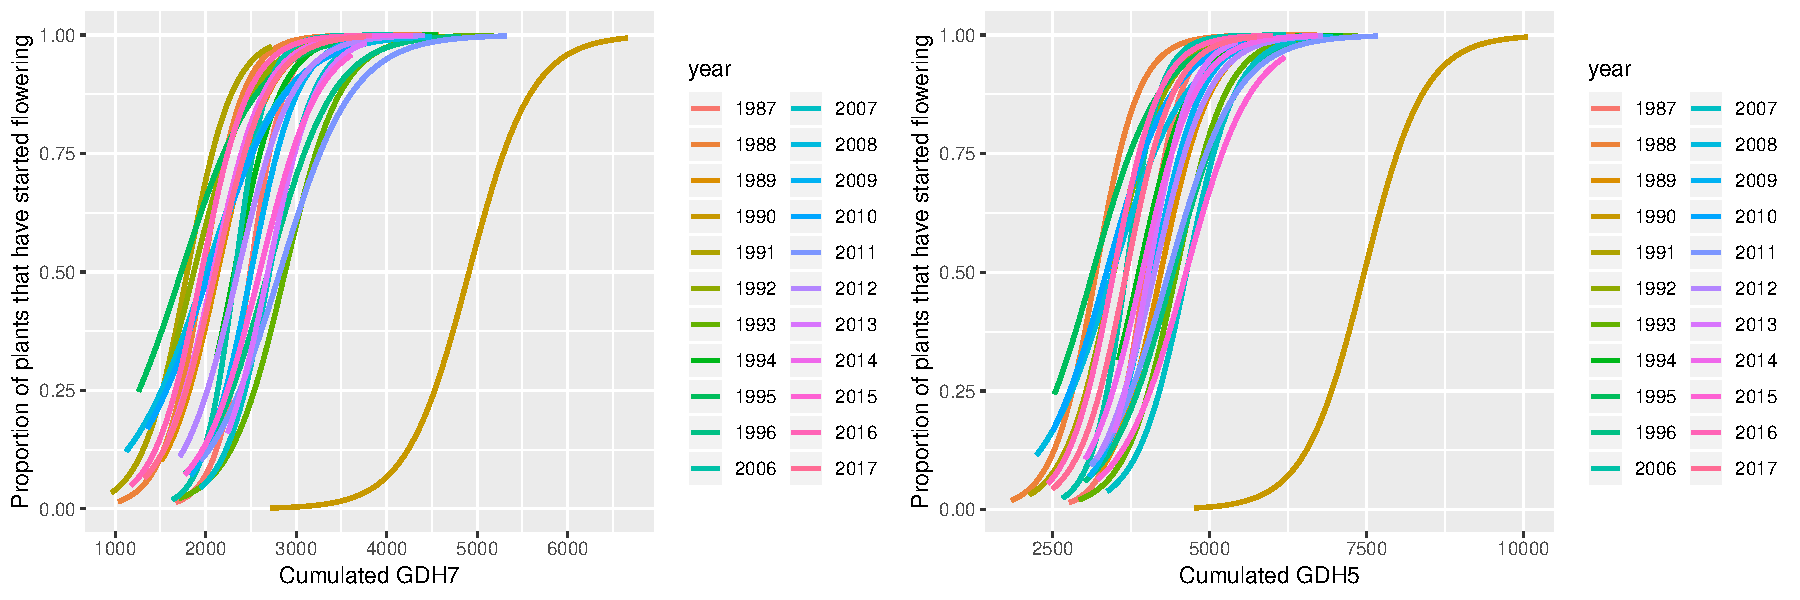
\includegraphics{weather_nb_files/figure-latex/Plots of proportion of plants starting flowering against cumulated GDD/GDH 1-1.pdf}

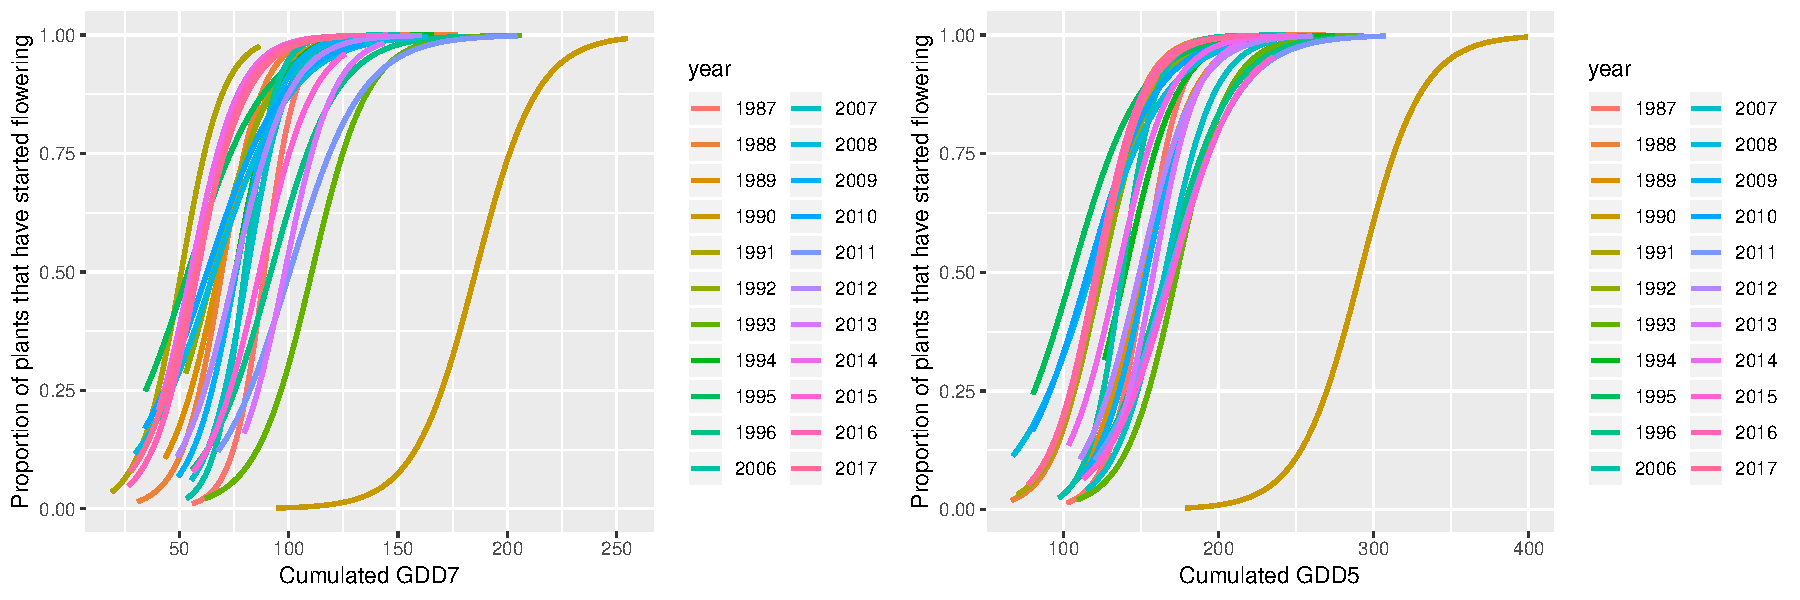
\includegraphics{weather_nb_files/figure-latex/Plots of proportion of plants starting flowering against cumulated GDD/GDH 2-1.pdf}

Year 1990 shows high values of GDD/GDH\\
Some plots to look at these high values

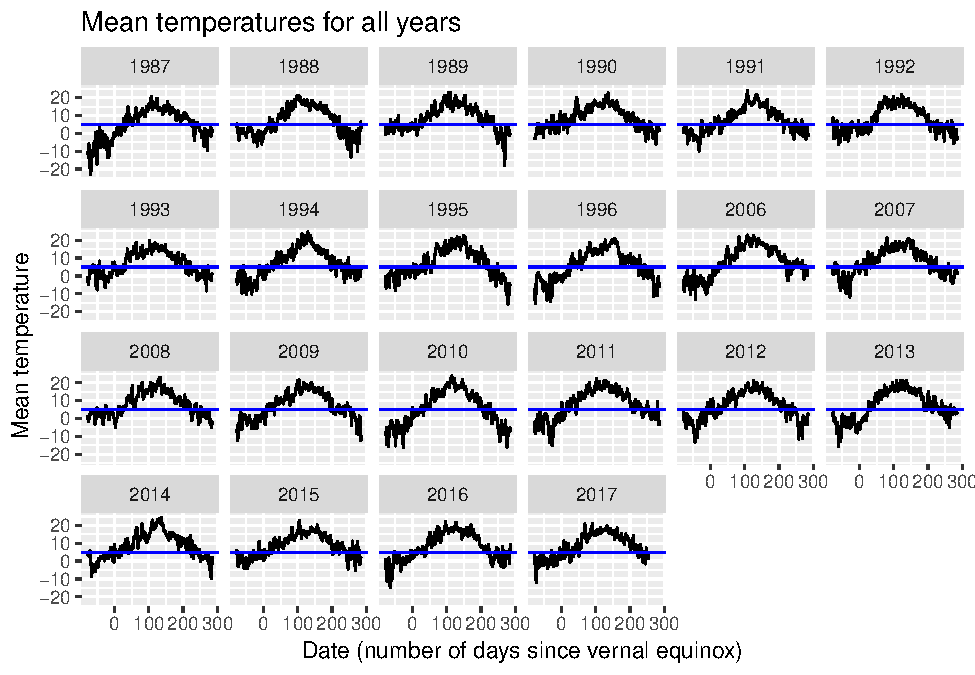
\includegraphics{weather_nb_files/figure-latex/1990-1.pdf}
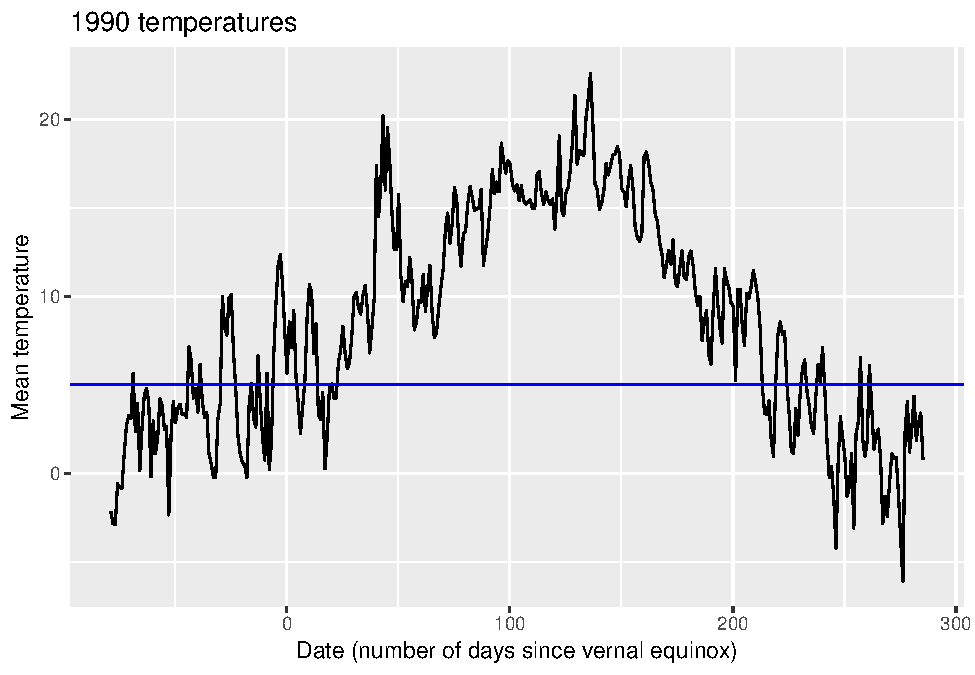
\includegraphics{weather_nb_files/figure-latex/1990-2.pdf}
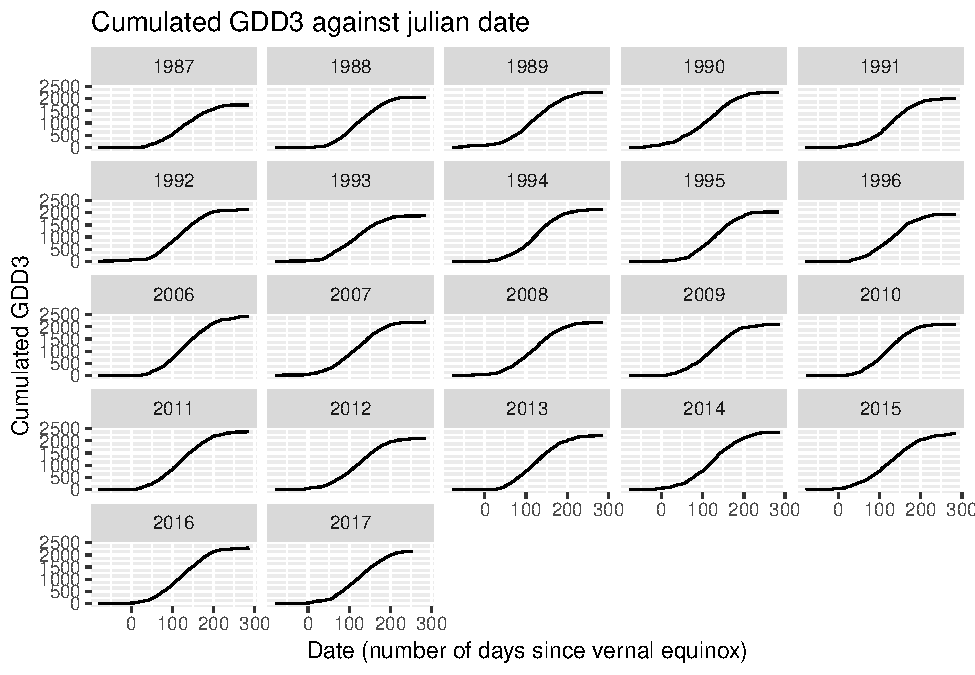
\includegraphics{weather_nb_files/figure-latex/1990-3.pdf}
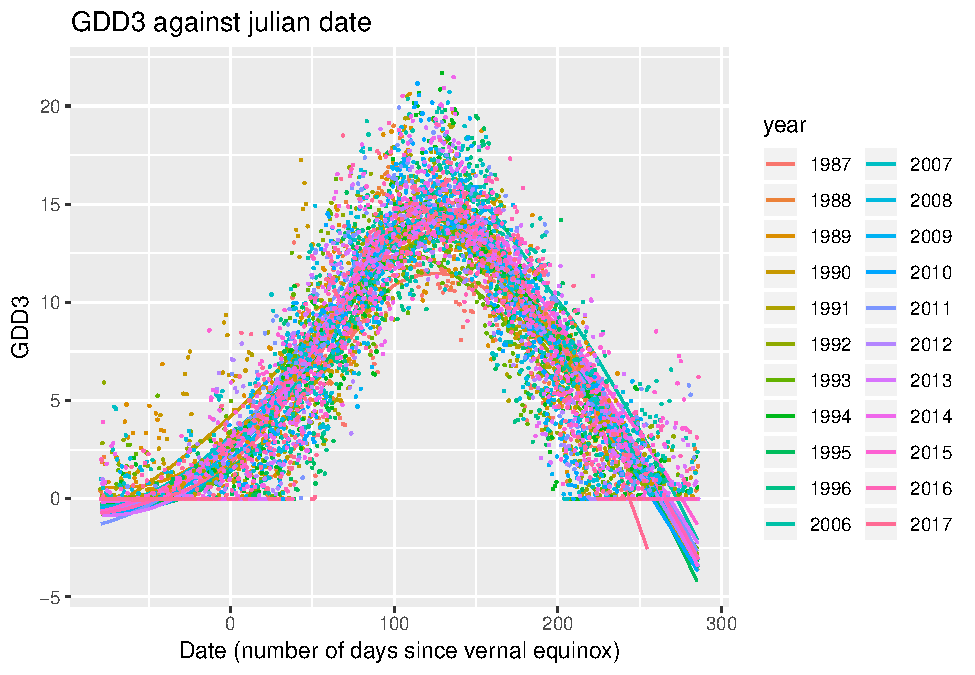
\includegraphics{weather_nb_files/figure-latex/1990-4.pdf}
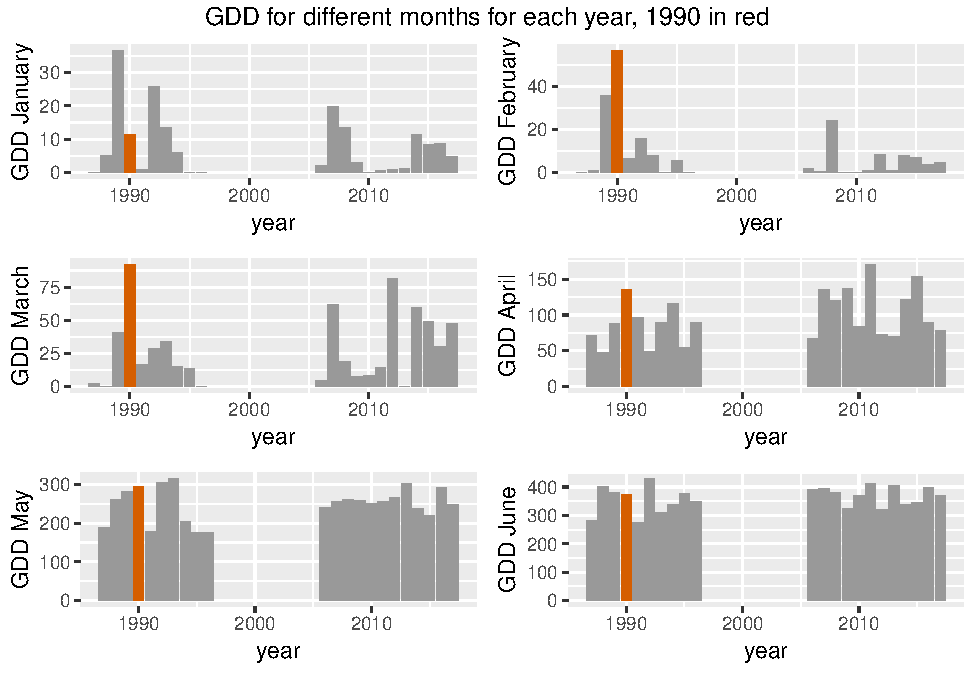
\includegraphics{weather_nb_files/figure-latex/1990-5.pdf}
\includegraphics{weather_nb_files/figure-latex/1990-6.pdf}
\includegraphics{weather_nb_files/figure-latex/1990-7.pdf}

GDD are very high in February and March 1990 - many days above the base
temperature in these months.

\newpage

Chilling temperatures in winter\\
Calculate number of days with temperatures below 0 / -5 during winter
(winter = 1st of December -- day before vernal equinox), as well as mean
temperatures and precipitation

\begin{Shaded}
\begin{Highlighting}[]
\NormalTok{weather}\OperatorTok{$}\NormalTok{winter<-}\KeywordTok{as.factor}\NormalTok{(}\KeywordTok{with}\NormalTok{(weather,}\KeywordTok{ifelse}\NormalTok{(month}\OperatorTok{==}\DecValTok{12}\OperatorTok{|}\NormalTok{period}\OperatorTok{==}\StringTok{"a"}\NormalTok{,}\DecValTok{1}\NormalTok{,}\DecValTok{0}\NormalTok{)))}
\CommentTok{#Define winter (=December or January-March till day before vernal equinox)}
\end{Highlighting}
\end{Shaded}

\begin{Shaded}
\begin{Highlighting}[]
\NormalTok{weather}\OperatorTok{$}\NormalTok{mean_below_}\DecValTok{0}\NormalTok{<-}\KeywordTok{with}\NormalTok{(weather,}\KeywordTok{ifelse}\NormalTok{(mean}\OperatorTok{<}\DecValTok{0}\NormalTok{,}\DecValTok{1}\NormalTok{,}\DecValTok{0}\NormalTok{))}
\NormalTok{weather}\OperatorTok{$}\NormalTok{min_below_}\DecValTok{0}\NormalTok{<-}\KeywordTok{with}\NormalTok{(weather,}\KeywordTok{ifelse}\NormalTok{(min}\OperatorTok{<}\DecValTok{0}\NormalTok{,}\DecValTok{1}\NormalTok{,}\DecValTok{0}\NormalTok{))}
\NormalTok{weather}\OperatorTok{$}\NormalTok{max_below_}\DecValTok{0}\NormalTok{<-}\KeywordTok{with}\NormalTok{(weather,}\KeywordTok{ifelse}\NormalTok{(max}\OperatorTok{<}\DecValTok{0}\NormalTok{,}\DecValTok{1}\NormalTok{,}\DecValTok{0}\NormalTok{))}
\NormalTok{weather}\OperatorTok{$}\NormalTok{mean_below_minus5<-}\KeywordTok{with}\NormalTok{(weather,}\KeywordTok{ifelse}\NormalTok{(mean}\OperatorTok{<}\NormalTok{(}\OperatorTok{-}\DecValTok{5}\NormalTok{),}\DecValTok{1}\NormalTok{,}\DecValTok{0}\NormalTok{))}
\NormalTok{weather}\OperatorTok{$}\NormalTok{min_below_minus5<-}\KeywordTok{with}\NormalTok{(weather,}\KeywordTok{ifelse}\NormalTok{(min}\OperatorTok{<}\NormalTok{(}\OperatorTok{-}\DecValTok{5}\NormalTok{),}\DecValTok{1}\NormalTok{,}\DecValTok{0}\NormalTok{))}
\NormalTok{weather}\OperatorTok{$}\NormalTok{max_below_minus5<-}\KeywordTok{with}\NormalTok{(weather,}\KeywordTok{ifelse}\NormalTok{(max}\OperatorTok{<}\NormalTok{(}\OperatorTok{-}\DecValTok{5}\NormalTok{),}\DecValTok{1}\NormalTok{,}\DecValTok{0}\NormalTok{))}

\NormalTok{mean_weather3_w<-}\KeywordTok{join_all}\NormalTok{(}\KeywordTok{list}\NormalTok{(}
    \KeywordTok{aggregate}\NormalTok{(mean }\OperatorTok{~}\StringTok{ }\NormalTok{year, }\DataTypeTok{data=}\KeywordTok{subset}\NormalTok{(weather,winter}\OperatorTok{==}\DecValTok{1}\NormalTok{), }\DataTypeTok{FUN=}\NormalTok{mean),   }\CommentTok{#Mean of mean daily temperature}
    \KeywordTok{aggregate}\NormalTok{(min }\OperatorTok{~}\StringTok{ }\NormalTok{year, }\DataTypeTok{data=}\KeywordTok{subset}\NormalTok{(weather,winter}\OperatorTok{==}\DecValTok{1}\NormalTok{), }\DataTypeTok{FUN=}\NormalTok{mean),    }\CommentTok{#Mean of min daily temperature}
    \KeywordTok{aggregate}\NormalTok{(max }\OperatorTok{~}\StringTok{ }\NormalTok{year, }\DataTypeTok{data=}\KeywordTok{subset}\NormalTok{(weather,winter}\OperatorTok{==}\DecValTok{1}\NormalTok{), }\DataTypeTok{FUN=}\NormalTok{mean),    }\CommentTok{#Mean of max daily temperature}
    \KeywordTok{aggregate}\NormalTok{(precipitation }\OperatorTok{~}\StringTok{ }\NormalTok{year, }\DataTypeTok{data=} \KeywordTok{subset}\NormalTok{(weather,winter}\OperatorTok{==}\DecValTok{1}\NormalTok{), }\DataTypeTok{FUN=}\NormalTok{sum),}\CommentTok{#Sum of precipitation}
    \KeywordTok{aggregate}\NormalTok{(mean_below_}\DecValTok{0} \OperatorTok{~}\StringTok{ }\NormalTok{year,}\DataTypeTok{data=} \KeywordTok{subset}\NormalTok{(weather,winter}\OperatorTok{==}\DecValTok{1}\NormalTok{), }\DataTypeTok{FUN=}\NormalTok{sum),  }\CommentTok{#N days with mean<0}
    \KeywordTok{aggregate}\NormalTok{(min_below_}\DecValTok{0} \OperatorTok{~}\StringTok{ }\NormalTok{year,}\DataTypeTok{data=} \KeywordTok{subset}\NormalTok{(weather,winter}\OperatorTok{==}\DecValTok{1}\NormalTok{), }\DataTypeTok{FUN=}\NormalTok{sum),  }\CommentTok{#N days with min<0}
    \KeywordTok{aggregate}\NormalTok{(max_below_}\DecValTok{0} \OperatorTok{~}\StringTok{ }\NormalTok{year,}\DataTypeTok{data=} \KeywordTok{subset}\NormalTok{(weather,winter}\OperatorTok{==}\DecValTok{1}\NormalTok{), }\DataTypeTok{FUN=}\NormalTok{sum),  }\CommentTok{#N days with max<0}
    \KeywordTok{aggregate}\NormalTok{(mean_below_minus5 }\OperatorTok{~}\StringTok{ }\NormalTok{year,}\DataTypeTok{data=} \KeywordTok{subset}\NormalTok{(weather,winter}\OperatorTok{==}\DecValTok{1}\NormalTok{), }\DataTypeTok{FUN=}\NormalTok{sum), }\CommentTok{#N days with mean<-5}
    \KeywordTok{aggregate}\NormalTok{(min_below_minus5 }\OperatorTok{~}\StringTok{ }\NormalTok{year,}\DataTypeTok{data=} \KeywordTok{subset}\NormalTok{(weather,winter}\OperatorTok{==}\DecValTok{1}\NormalTok{), }\DataTypeTok{FUN=}\NormalTok{sum),  }\CommentTok{#N days with min<-5}
    \KeywordTok{aggregate}\NormalTok{(max_below_minus5 }\OperatorTok{~}\StringTok{ }\NormalTok{year,}\DataTypeTok{data=} \KeywordTok{subset}\NormalTok{(weather,winter}\OperatorTok{==}\DecValTok{1}\NormalTok{), }\DataTypeTok{FUN=}\NormalTok{sum)), }\CommentTok{#N days with max<-5}
    \DataTypeTok{by =} \OtherTok{NULL}\NormalTok{, }\DataTypeTok{type =} \StringTok{"left"}\NormalTok{, }\DataTypeTok{match =} \StringTok{"all"}\NormalTok{)}
\end{Highlighting}
\end{Shaded}

\begin{verbatim}
## Joining by: year
## Joining by: year
## Joining by: year
## Joining by: year
## Joining by: year
## Joining by: year
## Joining by: year
## Joining by: year
## Joining by: year
\end{verbatim}

\begin{Shaded}
\begin{Highlighting}[]
\KeywordTok{colnames}\NormalTok{(mean_weather3_w)[}\DecValTok{2}\OperatorTok{:}\DecValTok{11}\NormalTok{]<-}\KeywordTok{paste}\NormalTok{(}\KeywordTok{colnames}\NormalTok{(mean_weather3_w)[}\DecValTok{2}\OperatorTok{:}\DecValTok{11}\NormalTok{],}\StringTok{"w"}\NormalTok{, }\DataTypeTok{sep =} \StringTok{"_"}\NormalTok{)}

\NormalTok{mean_weather4<-}\KeywordTok{merge}\NormalTok{(mean_weather3,mean_weather3_w) }\CommentTok{#Merge with previous data}
\end{Highlighting}
\end{Shaded}

Models FFD against winter variables

\begin{Shaded}
\begin{Highlighting}[]
\CommentTok{#Fit univariate linear models of FFD against each predictor}
\NormalTok{models2<-}\KeywordTok{lapply}\NormalTok{(}\KeywordTok{names}\NormalTok{(mean_weather4)[}\KeywordTok{c}\NormalTok{(}\DecValTok{219}\OperatorTok{:}\DecValTok{228}\NormalTok{)], }\ControlFlowTok{function}\NormalTok{(x) \{}
  \KeywordTok{summary}\NormalTok{(}\KeywordTok{lm}\NormalTok{(}\KeywordTok{substitute}\NormalTok{(FFD }\OperatorTok{~}\StringTok{ }\KeywordTok{scale}\NormalTok{(i), }\KeywordTok{list}\NormalTok{(}\DataTypeTok{i =} \KeywordTok{as.name}\NormalTok{(x))), }\DataTypeTok{data =}\NormalTok{ mean_weather4, }\DataTypeTok{na.action=}\NormalTok{na.exclude))}
\NormalTok{\})}

\CommentTok{#Build a table with estimate, p and r square for all fitted models}
\NormalTok{models2<-}\KeywordTok{cbind}\NormalTok{(}\KeywordTok{names}\NormalTok{(mean_weather4)[}\KeywordTok{c}\NormalTok{(}\DecValTok{219}\OperatorTok{:}\DecValTok{228}\NormalTok{)],}
              \KeywordTok{ldply}\NormalTok{(models2, }\ControlFlowTok{function}\NormalTok{(x) }\KeywordTok{coef}\NormalTok{(x)[}\DecValTok{2}\NormalTok{]),}
              \KeywordTok{ldply}\NormalTok{(models2, }\ControlFlowTok{function}\NormalTok{(x) }\KeywordTok{coef}\NormalTok{(x)[}\DecValTok{8}\NormalTok{]),}
              \KeywordTok{ldply}\NormalTok{(models2, }\ControlFlowTok{function}\NormalTok{(x) x}\OperatorTok{$}\NormalTok{adj.r.square)}
\NormalTok{      )}
\KeywordTok{names}\NormalTok{(models2)<-}\KeywordTok{c}\NormalTok{(}\StringTok{"variable"}\NormalTok{,}\StringTok{"estimate"}\NormalTok{,}\StringTok{"p"}\NormalTok{,}\StringTok{"adj.rsquare"}\NormalTok{)}
\NormalTok{models2}\OperatorTok{$}\NormalTok{sig<-}\KeywordTok{ifelse}\NormalTok{(models2}\OperatorTok{$}\NormalTok{p}\OperatorTok{<}\FloatTok{0.05}\NormalTok{,}\StringTok{"*"}\NormalTok{,}\StringTok{""}\NormalTok{) }\CommentTok{# *=p<0.05}

\CommentTok{#Order models by R square}
\KeywordTok{kable}\NormalTok{(}\KeywordTok{arrange}\NormalTok{(models2,}\KeywordTok{desc}\NormalTok{(adj.rsquare)))}
\end{Highlighting}
\end{Shaded}

\begin{longtable}[]{@{}lrrrl@{}}
\toprule
variable & estimate & p & adj.rsquare & sig\tabularnewline
\midrule
\endhead
precipitation\_w & -3.665808 & 0.0019909 & 0.3564066 & *\tabularnewline
mean\_w & -3.324004 & 0.0062438 & 0.2841524 & *\tabularnewline
max\_w & -3.287951 & 0.0069619 & 0.2769429 & *\tabularnewline
min\_w & -3.286051 & 0.0070015 & 0.2765653 & *\tabularnewline
min\_below\_0\_w & 3.234009 & 0.0081628 & 0.2663034 & *\tabularnewline
mean\_below\_0\_w & 3.100545 & 0.0118830 & 0.2407351 & *\tabularnewline
min\_below\_minus5\_w & 2.970477 & 0.0167406 & 0.2168540 &
*\tabularnewline
max\_below\_minus5\_w & 2.865391 & 0.0217429 & 0.1983071 &
*\tabularnewline
max\_below\_0\_w & 2.676526 & 0.0336962 & 0.1666529 & *\tabularnewline
mean\_below\_minus5\_w & 2.625453 & 0.0376865 & 0.1584634 &
*\tabularnewline
\bottomrule
\end{longtable}

More precipitation and higher temperatures in winter are correlated with
earlier flowering.\\
More cold days in winter is correlated with later flowering.

Does winter temperature/precipitation influence the response of plants
to spring temperature?\\
Do fewer days with freezing temperatures/warmer temperatures in winter
mean lower sensitivity to increasing spring temperatures?\\
Sensitivity to increasing spring temperatures for each year: calculated
as the coefficients from yearly models of proportion of plants having
started flowering against cumulated number of GDH3 (computed from the
vernal equinox) (This was the variable explaining the most variance in
the proportion of plants having started flowering)

\begin{Shaded}
\begin{Highlighting}[]
\CommentTok{#Proportion of plants having started flowering}
\NormalTok{models3<-}\KeywordTok{with}\NormalTok{(alldata_agg,}
            \KeywordTok{by}\NormalTok{(alldata_agg, year,}
               \ControlFlowTok{function}\NormalTok{(x) }\KeywordTok{glm}\NormalTok{(prop_fl }\OperatorTok{~}\StringTok{ }\NormalTok{cumGDH3v, }\DataTypeTok{data =}\NormalTok{ x,}\DataTypeTok{family=}\NormalTok{binomial)))}
\NormalTok{coefs_models3<-}\KeywordTok{as.data.frame}\NormalTok{(}\KeywordTok{sapply}\NormalTok{(models3, coef)[}\DecValTok{2}\NormalTok{,])}
\NormalTok{coefs_models3}\OperatorTok{$}\NormalTok{year<-}\KeywordTok{row.names}\NormalTok{(coefs_models3)}
\KeywordTok{names}\NormalTok{(coefs_models3)<-}\KeywordTok{c}\NormalTok{(}\StringTok{"resp_cumGDH3v"}\NormalTok{,}\StringTok{"year"}\NormalTok{)}

\NormalTok{mean_weather5<-}\KeywordTok{merge}\NormalTok{(mean_weather4,coefs_models3)}

\CommentTok{#Fit univariate linear models of resp_cumGDH3v against each winter predictor}
\NormalTok{models4<-}\KeywordTok{lapply}\NormalTok{(}\KeywordTok{names}\NormalTok{(mean_weather5)[}\KeywordTok{c}\NormalTok{(}\DecValTok{219}\OperatorTok{:}\DecValTok{228}\NormalTok{)], }\ControlFlowTok{function}\NormalTok{(x) \{}
  \KeywordTok{summary}\NormalTok{(}\KeywordTok{lm}\NormalTok{(}\KeywordTok{substitute}\NormalTok{(resp_cumGDH3v }\OperatorTok{~}\StringTok{ }\KeywordTok{scale}\NormalTok{(i), }\KeywordTok{list}\NormalTok{(}\DataTypeTok{i =} \KeywordTok{as.name}\NormalTok{(x))), }\DataTypeTok{data =}\NormalTok{ mean_weather5, }\DataTypeTok{na.action=}\NormalTok{na.exclude))}
\NormalTok{\})}

\CommentTok{#Build a table with estimate, p and r square for all fitted models}
\NormalTok{models4<-}\KeywordTok{cbind}\NormalTok{(}\KeywordTok{names}\NormalTok{(mean_weather5)[}\KeywordTok{c}\NormalTok{(}\DecValTok{219}\OperatorTok{:}\DecValTok{228}\NormalTok{)],}
              \KeywordTok{ldply}\NormalTok{(models4, }\ControlFlowTok{function}\NormalTok{(x) }\KeywordTok{coef}\NormalTok{(x)[}\DecValTok{2}\NormalTok{]),}
              \KeywordTok{ldply}\NormalTok{(models4, }\ControlFlowTok{function}\NormalTok{(x) }\KeywordTok{coef}\NormalTok{(x)[}\DecValTok{8}\NormalTok{]),}
              \KeywordTok{ldply}\NormalTok{(models4, }\ControlFlowTok{function}\NormalTok{(x) x}\OperatorTok{$}\NormalTok{adj.r.square)}
\NormalTok{      )}
\KeywordTok{names}\NormalTok{(models4)<-}\KeywordTok{c}\NormalTok{(}\StringTok{"variable"}\NormalTok{,}\StringTok{"estimate"}\NormalTok{,}\StringTok{"p"}\NormalTok{,}\StringTok{"adj.rsquare"}\NormalTok{)}
\NormalTok{models4}\OperatorTok{$}\NormalTok{sig<-}\KeywordTok{ifelse}\NormalTok{(models4}\OperatorTok{$}\NormalTok{p}\OperatorTok{<}\FloatTok{0.05}\NormalTok{,}\StringTok{"*"}\NormalTok{,}\StringTok{""}\NormalTok{) }\CommentTok{# *=p<0.05}

\CommentTok{#Order models by R square}
\KeywordTok{kable}\NormalTok{(}\KeywordTok{arrange}\NormalTok{(models4,}\KeywordTok{desc}\NormalTok{(adj.rsquare)))}
\end{Highlighting}
\end{Shaded}

\begin{longtable}[]{@{}lrrrl@{}}
\toprule
variable & estimate & p & adj.rsquare & sig\tabularnewline
\midrule
\endhead
precipitation\_w & -0.0001855 & 0.0166639 & 0.2171773 & *\tabularnewline
mean\_below\_0\_w & 0.0000915 & 0.2641913 & 0.0149978 &\tabularnewline
min\_w & -0.0000882 & 0.2820526 & 0.0104699 &\tabularnewline
min\_below\_minus5\_w & 0.0000872 & 0.2878224 & 0.0090796
&\tabularnewline
mean\_w & -0.0000790 & 0.3366843 & -0.0014774 &\tabularnewline
min\_below\_0\_w & 0.0000698 & 0.3972606 & -0.0121292 &\tabularnewline
max\_w & -0.0000632 & 0.4442198 & -0.0189611 &\tabularnewline
mean\_below\_minus5\_w & 0.0000572 & 0.4895856 & -0.0246136
&\tabularnewline
max\_below\_minus5\_w & 0.0000498 & 0.5475656 & -0.0307106
&\tabularnewline
max\_below\_0\_w & 0.0000471 & 0.5700600 & -0.0327793 &\tabularnewline
\bottomrule
\end{longtable}

It seems that only winter precipitation influences the response of
plants to increasing spring temperatures (with higher winter
precipitation, plants are less responsive to increasing spring
temperatures), and the effect is not very strong.\\
Another ways of testing this relation among winter conditions and
response to spring temperature: Models with effects of mean temperature
April and May, measures of chilling and their interaction on mean FFD.

\begin{Shaded}
\begin{Highlighting}[]
\CommentTok{#Fit linear models of FFD against mean45*chilling measure}
\NormalTok{models5<-}\KeywordTok{lapply}\NormalTok{(}\KeywordTok{names}\NormalTok{(mean_weather5)[}\KeywordTok{c}\NormalTok{(}\DecValTok{219}\OperatorTok{:}\DecValTok{228}\NormalTok{)], }\ControlFlowTok{function}\NormalTok{(x) \{}
  \KeywordTok{summary}\NormalTok{(}\KeywordTok{lm}\NormalTok{(}\KeywordTok{substitute}\NormalTok{(FFD }\OperatorTok{~}\StringTok{ }\KeywordTok{scale}\NormalTok{(mean45)}\OperatorTok{*}\KeywordTok{scale}\NormalTok{(i), }\KeywordTok{list}\NormalTok{(}\DataTypeTok{i =} \KeywordTok{as.name}\NormalTok{(x))), }
          \DataTypeTok{data =}\NormalTok{ mean_weather5, }\DataTypeTok{na.action=}\NormalTok{na.exclude))}
\NormalTok{\})}

\CommentTok{#Build a table with estimate, p and r square for all fitted models}
\NormalTok{models5<-}\KeywordTok{cbind}\NormalTok{(}\KeywordTok{names}\NormalTok{(mean_weather5)[}\KeywordTok{c}\NormalTok{(}\DecValTok{219}\OperatorTok{:}\DecValTok{228}\NormalTok{)],}
              \KeywordTok{ldply}\NormalTok{(models5, }\ControlFlowTok{function}\NormalTok{(x) }\KeywordTok{coef}\NormalTok{(x)[}\DecValTok{4}\NormalTok{]),}
              \KeywordTok{ldply}\NormalTok{(models5, }\ControlFlowTok{function}\NormalTok{(x) }\KeywordTok{coef}\NormalTok{(x)[}\DecValTok{16}\NormalTok{]),}
              \KeywordTok{ldply}\NormalTok{(models5, }\ControlFlowTok{function}\NormalTok{(x) x}\OperatorTok{$}\NormalTok{adj.r.square)}
\NormalTok{      )}
\KeywordTok{names}\NormalTok{(models5)<-}\KeywordTok{c}\NormalTok{(}\StringTok{"variable"}\NormalTok{,}\StringTok{"estimate"}\NormalTok{,}\StringTok{"p"}\NormalTok{,}\StringTok{"adj.rsquare"}\NormalTok{)}
\NormalTok{models5}\OperatorTok{$}\NormalTok{sig<-}\KeywordTok{ifelse}\NormalTok{(models5}\OperatorTok{$}\NormalTok{p}\OperatorTok{<}\FloatTok{0.05}\NormalTok{,}\StringTok{"*"}\NormalTok{,}\StringTok{""}\NormalTok{) }\CommentTok{# *=p<0.05}

\CommentTok{#Order models by R square}
\KeywordTok{kable}\NormalTok{(}\KeywordTok{arrange}\NormalTok{(models5,}\KeywordTok{desc}\NormalTok{(adj.rsquare)))}
\end{Highlighting}
\end{Shaded}

\begin{longtable}[]{@{}lrrrl@{}}
\toprule
variable & estimate & p & adj.rsquare & sig\tabularnewline
\midrule
\endhead
precipitation\_w & 0.8633909 & 0.2332496 & 0.7836344 &\tabularnewline
min\_below\_0\_w & -0.3015655 & 0.6826601 & 0.7593436 &\tabularnewline
max\_w & 0.5797146 & 0.4343327 & 0.7565030 &\tabularnewline
max\_below\_minus5\_w & -0.6100128 & 0.4447081 & 0.7540362
&\tabularnewline
mean\_w & 0.4149907 & 0.5612885 & 0.7532095 &\tabularnewline
mean\_below\_0\_w & -0.3261530 & 0.6774032 & 0.7505538 &\tabularnewline
min\_w & 0.2376274 & 0.7398845 & 0.7505072 &\tabularnewline
max\_below\_0\_w & -0.6363942 & 0.4837476 & 0.7479327 &\tabularnewline
min\_below\_minus5\_w & -0.2585940 & 0.7348488 & 0.7472340
&\tabularnewline
mean\_below\_minus5\_w & -0.4067785 & 0.6321929 & 0.7450429
&\tabularnewline
\bottomrule
\end{longtable}

Test this within years instead of among years?


\end{document}
